\documentclass[twoside]{article}
\usepackage{aistats2027}
\usepackage[round]{natbib}
\renewcommand{\bibname}{References}
\renewcommand{\bibsection}{\subsubsection*{\bibname}}
\usepackage{amsmath,amssymb,amsthm,mathtools}
\usepackage{booktabs,graphicx,xcolor,adjustbox}
\usepackage{tikz}
\usetikzlibrary{positioning,arrows.meta,fit,calc}
\usepackage[hidelinks]{hyperref}
\newtheorem{theorem}{Theorem}
\newtheorem{proposition}[theorem]{Proposition}
\newtheorem{lemma}[theorem]{Lemma}
\newtheorem{corollary}[theorem]{Corollary}
\newtheorem{conjecture}[theorem]{Conjecture}
\theoremstyle{definition}
\newtheorem{definition}[theorem]{Definition}
\newtheorem{assumption}{Assumption}
\theoremstyle{remark}
\newtheorem{remark}[theorem]{Remark}
\newtheorem{example}[theorem]{Example}

\newcommand{\Dfit}{D_{\mathrm{fit}}}
\newcommand{\Dcal}{D_{\mathrm{cal}}}
\newcommand{\Dtest}{D_{\mathrm{test}}}
\newcommand{\Info}{\mathcal{I}}
\newcommand{\E}{\mathbb{E}}
\renewcommand{\P}{\mathbb{P}}
\newcommand{\1}{\mathbf{1}}
\DeclareMathOperator{\diam}{diam}
\newcommand{\expname}[1]{\textsc{#1}}


\begin{document}

\twocolumn[

\aistatstitle{How Finely to Group? Learned Partitions for Calibrating LLM Confidence across Elicitation Procedures}

\aistatsauthor{ Anonymous Author(s) }

\aistatsaddress{ Anonymous Institution(s) } ]

\begin{abstract}
Language models report confidence that depends on how they are asked: rewording a prompt or reversing
a scale changes which answers look confident and breaks calibrations made under the original
procedure. We ask whether grouping question--answer pairs by a frozen representation computed before
elicitation provides calibration structure across elicitation procedures, and how finely to group under
a limited label budget. Across three open models, two factual question-answering datasets and synthetic
reliability models, groups improve on recalibrating the confidence report only when reliability differs
between groups and labels are plentiful (thousands of labelled questions, and even then the gain is
small); otherwise their estimation cost outweighs the benefit, and a direct predictor on the same
features does better. Groups do not shrink conformal prediction sets, and they do not remove the
dependence on the procedure, because the forecast still reads the report. A monotone map between two
procedures' reports, fitted without labels, carries a calibration across procedures on average but not
within every group. Calibration should therefore be checked, and reported, per prompt and scale.
\end{abstract}

\section{Introduction}
\label{sec:intro}
Asking a language model how confident it is costs one extra prompt, needs no access to weights, and
returns a number a person can read; systems use such reports to abstain, to escalate to a human, or to
trigger retrieval \citep{kadavath2022language,tian2023just,xiong2024can}. The report is calibrated to
correctness under the procedure used to elicit it --- a prompt, a scale, a legend that maps letters to
percentages --- and procedures change: prompts are edited, scales are reversed, templates are reworded.

\paragraph{A motivating observation.} A model reports confidence for a fixed candidate answer by
choosing a letter from A to L, read through a legend (A $=0\%$ \dots L $=100\%$). Reverse the legend
and decode through the reversed legend, and a calibration made under one legend should still hold under
the other. It does not (Figure~\ref{fig:overview}a, Table~\ref{tab:coverage}): on 7{,}189 PopQA questions, conformal
sets calibrated under the forward legend cover $0.49$ for Mistral-7B under the reversed legend and $0.50$ under a
reworded prompt, and $0.76$ for Llama-3.1-8B under reversal, against a target of $0.90$; a trained reporter falls
from $0.90$ to $0.20$; other models become needlessly conservative. The reports themselves reshuffle: on 817
TruthfulQA questions a typical question moves 190--240 rank positions under reversal, against 239 if the two
rankings were independent, and only 20--24\% stay in their confidence fifth (20\% by chance).

\begin{figure*}[t]
  \centering
  \resizebox{\textwidth}{!}{%
    % Main schematic (Figure 1). Drawn in TikZ to match the caption in main.tex.
% Needs \usepackage{tikz} and \usetikzlibrary{positioning,arrows.meta,fit,calc}.
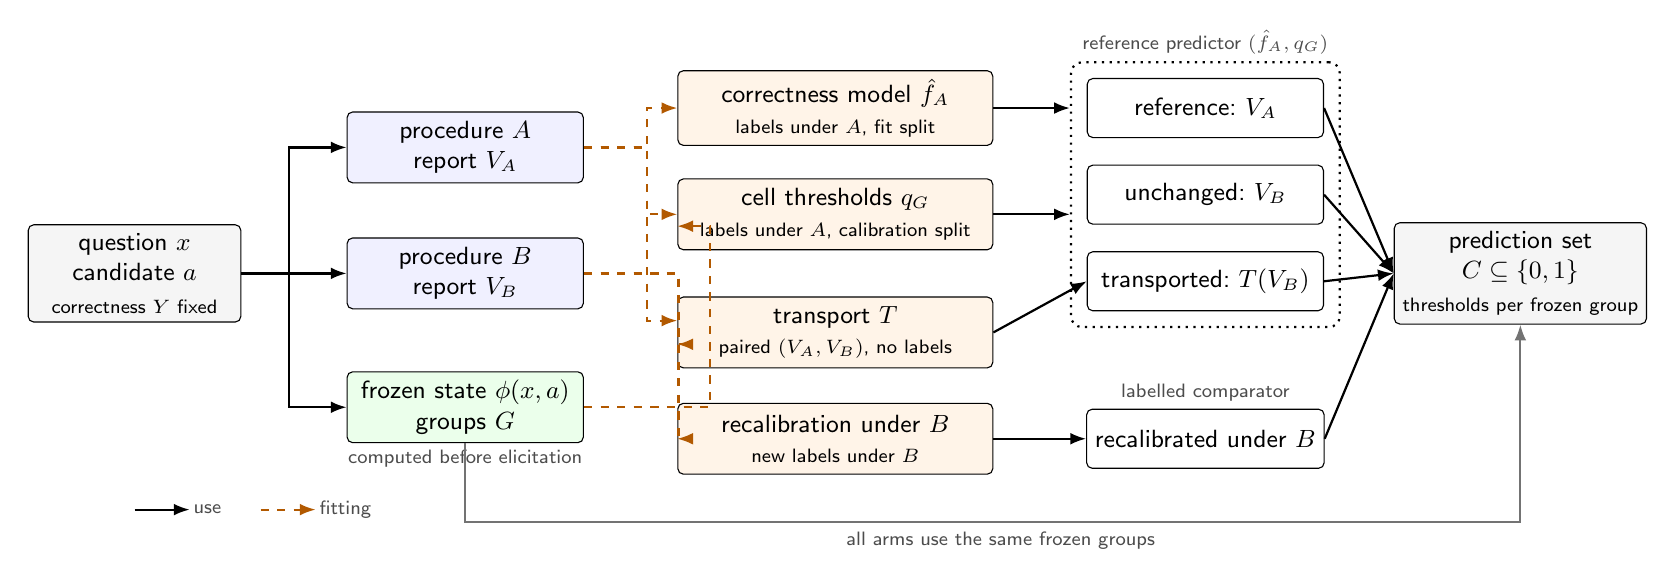
\begin{tikzpicture}[
  font=\sffamily\small,
  box/.style={draw, rounded corners=2pt, align=center, inner sep=3pt, minimum height=9mm, minimum width=30mm, fill=white},
  inbox/.style={box, fill=gray!8, minimum width=27mm},
  pbox/.style={box, fill=blue!6},
  gbox/.style={box, fill=green!8},
  fbox/.style={box, fill=orange!9, minimum width=40mm},
  abox/.style={box, minimum width=30mm, minimum height=7.5mm},
  use/.style={-{Latex[length=2mm]}, thick},
  fitarrow/.style={-{Latex[length=2mm]}, thick, dashed, orange!70!black},
  lbl/.style={font=\sffamily\scriptsize, inner sep=1pt, text=black!70}
]
% columns: inputs | procedures, groups | fitted objects | deployment arms | output
\node[inbox] (in) at (0,0) {question $x$\\candidate $a$\\[1pt]{\scriptsize correctness $Y$ fixed}};

\node[pbox] (A) at (4.2, 1.6) {procedure $A$\\report $V_A$};
\node[pbox] (B) at (4.2, 0)   {procedure $B$\\report $V_B$};
\node[gbox] (G) at (4.2,-1.7) {frozen state $\phi(x,a)$\\groups $G$};
\node[lbl, below=0.5mm of G] {computed before elicitation};

\node[fbox] (f) at (8.9, 2.1)  {correctness model $\hat f_A$\\{\scriptsize labels under $A$, fit split}};
\node[fbox] (q) at (8.9, 0.75) {cell thresholds $q_G$\\{\scriptsize labels under $A$, calibration split}};
\node[fbox] (T) at (8.9,-0.75) {transport $T$\\{\scriptsize paired $(V_A,V_B)$, no labels}};
\node[fbox] (R) at (8.9,-2.1)  {recalibration under $B$\\{\scriptsize new labels under $B$}};

\node[abox] (r1) at (13.6, 2.1)  {reference:\ $V_A$};
\node[abox] (r2) at (13.6, 1.0)  {unchanged:\ $V_B$};
\node[abox] (r3) at (13.6,-0.1)  {transported:\ $T(V_B)$};
\node[abox] (r4) at (13.6,-2.1)  {recalibrated under $B$};
\node[draw, dotted, thick, rounded corners, fit=(r1)(r2)(r3), inner sep=2mm] (ref) {};
\node[lbl, above=0.5mm of ref] {reference predictor $(\hat f_A, q_G)$};
\node[lbl, above=0.5mm of r4] {labelled comparator};

\node[box, fill=gray!8, minimum width=24mm] (out) at (17.6, 0) {prediction set\\$C\subseteq\{0,1\}$\\[1pt]{\scriptsize thresholds per frozen group}};

% elicitation
\draw[use] (in.east) -- ++(0.6,0) |- (A.west);
\draw[use] (in.east) -- (B.west);
\draw[use] (in.east) -- ++(0.6,0) |- (G.west);

% fitting (dashed)
\draw[fitarrow] (A.east) -- ++(0.8,0) |- (f.west);
\draw[fitarrow] (A.east) -- ++(0.8,0) |- (q.west);
\draw[fitarrow] (G.east) -- ++(1.6,0) |- ([yshift=-1.5mm]q.west);
\draw[fitarrow] (A.east) -- ++(0.8,0) |- ([yshift=1.5mm]T.west);
\draw[fitarrow] (B.east) -- ++(1.2,0) |- ([yshift=-1.5mm]T.west);
\draw[fitarrow] (B.east) -- ++(1.2,0) |- (R.west);

% deployment
\draw[use] (f.east) -- (ref.west |- f.east);
\draw[use] (q.east) -- (ref.west |- q.east);
\draw[use] (T.east) -- (r3.west);
\draw[use] (R.east) -- (r4.west);
\foreach \r in {r1,r2,r3,r4} \draw[use] (\r.east) -- (out.west);
\draw[use, black!55] (G.south) -- ++(0,-1.0) -| (out.south);
\node[lbl, fill=white] at (11.0,-3.4) {all arms use the same frozen groups};

% legend
\draw[use] (0.0,-3.0) -- ++(0.7,0) node[right, lbl] {use};
\draw[fitarrow] (1.6,-3.0) -- ++(0.7,0) node[right, lbl] {fitting};
\end{tikzpicture}
%
  }
  \caption{\textbf{Calibrating and transporting confidence reports.}
  The question, candidate and correctness remain fixed while the
  elicitation procedure changes. Labels under $A$ fit the correctness
  model and, on a separate calibration split, the cell thresholds.
  At deployment, the reference predictor receives $V_A$, unchanged
  $V_B$, or $T(V_B)$. Transport $T$ is fitted without correctness labels
  using paired reports for the same inputs. The labelled comparator
  instead recalibrates under $B$ using new labels. All arms use the same
  frozen groups and return prediction sets of correctness labels.
  Dashed arrows denote fitting.}
  \label{fig:main}
\end{figure*}

\begin{figure*}[t]
\centering
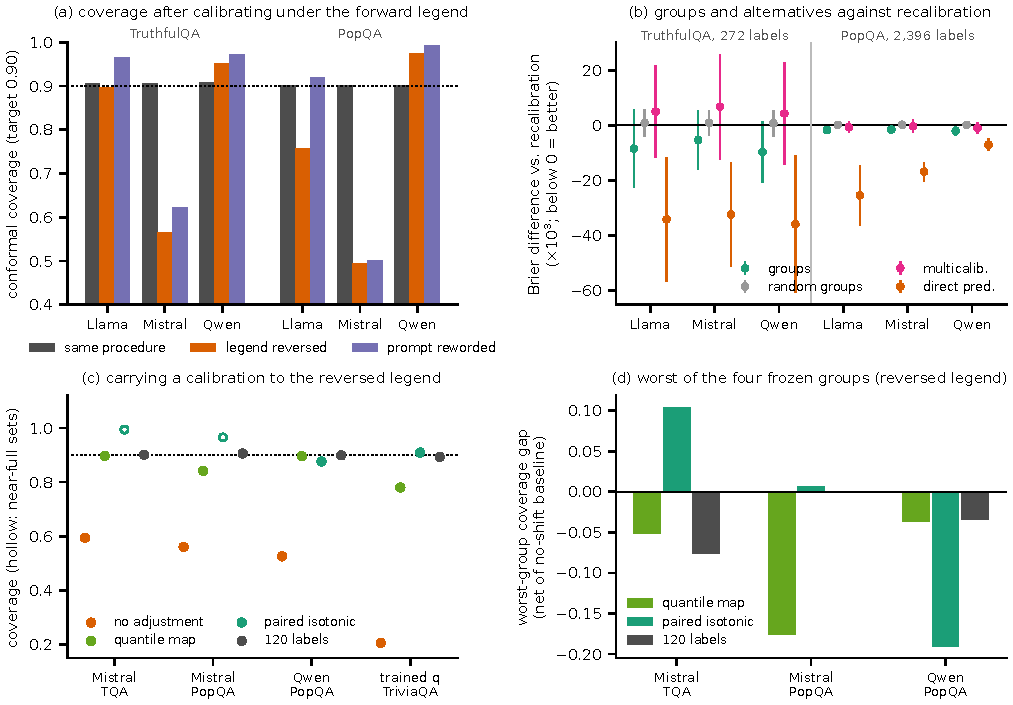
\includegraphics[width=\textwidth]{figs/fig_overview.pdf}
\caption{Overview. (a) Conformal coverage ($\alpha=0.1$, target dotted) when a calibration made under the
forward legend is deployed under the same legend, the reversed legend or a reworded prompt (three frozen
models; mean over 500 random splits; Table~\ref{tab:coverage}). (b) Brier difference against
procedure-specific recalibration ($\times10^3$; below zero: better) at the largest label budget, for learned
groups, random groups, multicalibration and a direct predictor on the same representation, with
Nadeau--Bengio-corrected 95\% intervals. (c) Coverage after carrying the calibration to the reversed legend:
no adjustment, two label-free maps fitted on unlabelled questions elicited both ways, and recalibration on
120 labelled questions under the new legend; hollow markers mark near-full sets (at least 1.9 of 2 labels).
(d) Coverage gap of the worst of the four frozen groups for the same arms, net of the same statistic with no
procedure change; below zero, a group is left short.}
\label{fig:overview}
\end{figure*}

\paragraph{Three questions.} One remedy recalibrates the report under each procedure, at a cost in labels per
procedure; the other groups question--answer examples by a frozen representation computed \emph{before}
elicitation and forecasts correctness from group and procedure together (Figure~\ref{fig:main}). The registered
question is when the second adds calibration structure beyond the first and when estimating more groups costs
more than it gains. It needs three answers: which groupings license a decision (Section~\ref{sec:validity}); how
finely to group under a label budget (Section~\ref{sec:decomp}; \expname{Granularity}, \expname{Synthetic-Reliability}); and
whether a calibration can be carried across procedures without new labels, since the groups do not move with
the procedure but a forecast built on them still reads the report (Proposition~\ref{prop:transport};
\expname{Label-Free-Transfer}).

\paragraph{Contributions.}
(i) A stage-indexed criterion for which groupings license a decision, synthesising known validity
results, and a label-free transport proposition: the coverage change from mapping one procedure's reports
onto another's is bounded by masses computable from unlabelled questions, and vanishes when the change is
monotone (Section~\ref{sec:validity}).
(ii) The granularity trade-off for conformal coverage with frozen groups: cell-averaged error depends on
counts only (Corollary~\ref{cor:B0}), the pointwise error splits into quantisation and estimation
(Proposition~\ref{prop:decomp}), and farthest-first cells admit a finite-sample bound (Lemma~\ref{lem:diam},
Theorem~\ref{thm:B}); for forecasts by group and procedure the split is a heuristic that the experiments test.
(iii) An answer to the registered question: against procedure-specific recalibration, multicalibration
and a direct predictor on the same features, groups help only where reliability varies between groups and
labels are plentiful (on PopQA, one of fifteen pre-declared tests at 2{,}396 labels; a gain of about 1--2\%
of the Brier score), the best granularity grows with the budget, a tuned direct predictor does better
throughout, groups do not shrink conformal sets, and groups do not protect calibration across a change of
procedure.
(iv) A transport phenomenon, studied in first experiments: a monotone map between paired reports repairs a
calibration on average, exactly when the change is monotone, but not per group (\expname{Label-Free-Transfer}).
Criteria were fixed in dated notes before each run, except where marked post hoc (Appendix~\ref{app:protocol});
\expname{PopQA-Elicit} and three other experiments were added after the TruthfulQA family returned no significant
group effect, and pooled with it (27 tests) no group-versus-recalibration test survives Holm correction. 

% ---------------------------------------------------------------------

\section{Setup}
\label{sec:setup}

\subsection{Stages of information}
Each unit is an independent draw of
\begin{gather*}
  W = (X, A, Y),\\
  \Info_0 = X,\quad \Info_1 = (X, A),\quad \Info_2 = (X, A, Y),
\end{gather*}
where $X$ is the input (prompt), $A$ is any randomness realised by the system
before the outcome is revealed (e.g.\ a sampled answer and its decoding seed),
and $Y$ is the outcome (e.g.\ correctness). A decision is \emph{taken at stage
$t$} if it may use $\Info_t$ but nothing later. The stage-$t$ nonconformity score
is $S = s(\Info_t, Y)$ and the prediction set is
$C(\Info_t) = \{y: s(\Info_t, y) \le q_{G}\}$ for a cell index $G$.

\subsection{Bins}
A bin is a cell indexed by a stored exemplar. The general
stage-$t$ binning is Definition~\ref{def:binning} in Appendix~\ref{app:binning}; every
result in Section~\ref{sec:validity} holds for it.

\begin{definition}[Exemplar cells]
\label{def:exemplar}
Given a feature map $\phi$ and exemplars $e_1,\dots,e_M$, all fitted on $\Dfit$ only,
$\gamma(x)=\arg\min_j \|\phi(x)-e_j\|$ (ties to the lower index). The balanced variant uses
power cells $\arg\min_j(\|\phi(x)-e_j\|^2-w_j)$ with weights $w$ fitted on $\Dfit$
. A residual cell $0$ collects queries outside every fitted radius
(Proposition~\ref{prop:D}). After fitting, the cell of a query depends on that query
alone (the \emph{write-free} condition).
\end{definition}

\subsection{Elicitation procedures and forecasters}
\label{sec:forecasters}
Each unit is $W=(X,\Pi,A,Y)$: the input, the elicitation procedure $\Pi$ (legend, prompt wording), the
system's own randomness, and the outcome. The report is $V=V_\Pi(X,A)$; a group $G=\gamma(\phi(X))$ is
computed from a frozen representation $\phi$ before any confidence prompt, so $G$ does not depend on
$\Pi$. Correctness forecasts are logistic in report, group and procedure,
\begin{equation}
  \mathrm{logit}\,\P(Y=1\mid V,G,\Pi=\pi) = a_\pi + b_\pi\,\mathrm{logit}\,V + c_{G,\pi},
  \label{eq:forecaster}
\end{equation}
with $c\equiv0$ for procedure-specific recalibration R, $c_{G,\pi}$ free for the group forecaster
G$_M$, and $c_{G,\pi}=c_G$ for offsets shared across procedures. For a fitted forecaster $\hat f$ and
$\eta^\star=\P(Y=1\mid V,Z,\Pi)$ with $Z$ the full frozen representation (which does not depend on $M$),
$\E(\hat f-Y)^2=\E[\eta^\star(1-\eta^\star)]+\E(\hat f-\eta^\star)^2$ exactly, and
$\E(\hat f-\eta^\star)^2\le2\,\E(f^\star-\eta^\star)^2+2\,\E(\hat f-f^\star)^2$ with $f^\star$ the best model of
the form~\eqref{eq:forecaster}. The approximation term falls as groups resolve reliability
differences; the estimation term grows roughly as the number of parameters, $|\Pi|(M+1)$ per
$n_{\mathrm{lab}}$ labels (a heuristic, not a bound). This
is the forecast-side analogue of the quantisation--estimation split of
Section~\ref{sec:decomp}; \expname{Granularity} tests it. Theorem~\ref{thm:B} concerns conformal pointwise coverage,
not these forecasts.

\subsection{Honest split and calibration rule}
$\Dfit$, $\Dcal$, $\Dtest$ are disjoint and sampled at the independent unit
(question id for LLM data; one variant per question). The score, feature map,
exemplars and cell rule are learned on $\Dfit$ alone. For cell $j$ with $n_j$
calibration scores, $t \coloneqq 1-\alpha$,
$k_j = \lceil (n_j+1)t \rceil$, and
\[
  q_j =
  \begin{cases}
    S_{(k_j)}^{(j)} & \text{if } k_j \le n_j \text{ and } n_j \ge n_{\min},\\
    +\infty & \text{otherwise (full set)}.
  \end{cases}
\]
The floor $n_{\min}$ is the same in every arm; test points in below-floor cells
are retained and the infinite-set mass is reported.

% ---------------------------------------------------------------------
\section{Which groupings license a decision}
\label{sec:validity}

\begin{theorem}[Per-cell validity]
\label{thm:A}
Fix $\Dfit$, hence $s$ and $\gamma$. Let the calibration units and the test unit be
exchangeable and independent of $\Dfit$, and let $G=\gamma(\Info_t)$. Then for every
cell $j$,
\[
  \P\{Y_{\mathrm{test}} \in C(\Info_{t,\mathrm{test}}) \mid G_{\mathrm{test}} = j\} \ \ge\ 1-\alpha,
\]
and if scores are a.s.\ distinct and $q_j<\infty$, the conditional coverage given $n_j$
is at most $1-\alpha + 1/(n_j+1)$.
\end{theorem}

\begin{proposition}[Stage measurability]
\label{prop:M-suff}
(A restatement of Mondrian validity, \citealp{vovk2012conditional}, and of selection
applied identically to calibration and test units, \citealp[Thm.~1]{bao2024selective}; the content
is the stage indexing.) If the decision is taken at stage $t$, the binning $\gamma$ is
$\Info_t$-measurable and frozen on $\Dfit$, the score is $s(\Info_t,Y)$, and calibration and
test units are retained by the same fixed $\Info_t$-measurable event $E$ (possibly trivial),
then the guarantee of Theorem~\ref{thm:A} holds for the stage-$t$ decision, conditional on $E$.
\end{proposition}

Outcome selection breaks coverage (Example~\ref{ex:M-fail}, Appendix~\ref{app:theory}): calibrating on the
answerable set and testing on the full stream gives coverage $p\,t$, where $p$ is the answerable share,
in the model of that example; answer-computed confidence licenses
post-generation decisions only (Remark~\ref{rem:vc}).

\paragraph{The stage criterion.} We call Proposition~\ref{prop:M-suff} together with its three
failure modes the \emph{stage criterion}: a grouping licenses a decision only if it is computable
from what is known at that decision, is not selected on the outcome (Example~\ref{ex:M-fail}),
and is applied under the elicitation convention it was calibrated in (Remark~\ref{rem:vc}; \expname{Elicitation-Shift}).

\paragraph{Transporting a calibration across procedures.} The stage criterion says a calibration
fitted under procedure A is not licensed under B. Because a question can be elicited under both
procedures without being labelled, the coupling of $(V_A,V_B)$ is observable, and a label-free map
$T$ can carry B's reports back to A's scale. Let $C_A$ be the conformal set computed from $V_A$ with
A's forecaster, thresholds and frozen group, and $C_T$ the set computed in the same way from
$T(V_B)$.

\begin{proposition}[Label-free transport]
\label{prop:transport}
(a) For any map $T$, $|\P(Y\in C_T)-\P(Y\in C_A)|\le\P(C_T\ne C_A)$, and the same holds within each
frozen group. The right-hand side, the \emph{crossing mass}, depends only on $(V_A,V_B,G)$, so it can
be estimated from unlabelled questions elicited under both procedures. One-sidedly, conditionally on
the calibration data and on $T$, $\P(Y\in C_T)\ge\P(Y\in C_A)-\ell$ with the \emph{label-loss mass}
$\ell=\P(C_A\not\subseteq C_T)$, which again needs no labels; averaging over the calibration draw and using
$\P(Y\in C_A)\ge1-\alpha$ gives $\P(Y\in C_T)\ge1-\alpha-\E\ell$. Both statements assume the outcome $Y$ is
the same under both procedures, which holds when the question and candidate are fixed. If $\hat\ell$ is the
label-loss rate on $m$ unlabelled questions independent of the calibration data and of the fold that fits
$T$, then $\ell\le\hat\ell+\sqrt{\log(1/\delta)/(2m)}$ with probability at least $1-\delta$ given those, so the
coverage under B is at most $\hat\ell+\sqrt{\log(1/\delta)/(2m)}$ below that under A; a union bound covers
several maps or groups.
(b) If $V_B=g(V_A)$ almost surely for a strictly monotone $g$, the population isotonic regression of
$V_A$ on $V_B$ (in the direction that fits) equals $g^{-1}$, so $C_T=C_A$ and the guarantee of
Theorem~\ref{thm:A}, per frozen group, transfers to B without labels. If $g$ is increasing and the
laws are continuous, the quantile map $F_A^{-1}\circ F_B$, the monotone optimal-transport map between
the two marginals, also equals $g^{-1}$.
(c) For continuous laws with finite second moments, the observed coupling of $(V_A,V_B)$ is comonotone, i.e.\ (b) holds with $g$
increasing, if and only if its squared-cost transport equals the optimal value $W_2^2$ between the
two marginals; the gap between the realised and optimal transport costs measures the departure
from a monotone change.
\end{proposition}

Groups computed before elicitation do not move with $\Pi$, which is what lets the per-group
statements in (a)--(b) be used across procedures.

% ---------------------------------------------------------------------
\section{Estimands: pointwise versus cell level}
\label{sec:estimands}
Our primary estimand is the pointwise (conditional-on-$X$) coverage gap.

Fix $\Dfit$ and $\Dcal$. Let $h(x) = F_x(q_{\gamma(x)})$, with $F_x$ the conditional score
CDF, $p_j=\P(\gamma(X)=j)$ and $C_j = \E[h(X)\mid\gamma(X)=j]$.
\begin{itemize}
  \item pointwise gap: $R_{\mathrm{pt}} = \E_X[(h(X)-t)^2]$;
  \item cell MSCE: $R_{\mathrm{cell}} = \textstyle\sum_j p_j (C_j-t)^2$;
  \item spread: $\max_j C_j - \min_j C_j$;
  \item concentrated undercoverage: $\max_{j:\,q_j<\infty} (t-C_j)_+$, eligible only if the full-set
  test mass is at most $1\%$.
\end{itemize}

\begin{corollary}[Cell-averaged MSCE is blind to heterogeneity]
\label{cor:B0}
An aggregation of the per-cell Beta law \citep{vovk2012conditional,ding2023class}. Assume continuous within-cell score CDFs and condition on the counts $(n_j)$ with
$n_{\min}\le n_j$ and $k_j\le n_j$ for all $j$. Then $C_j\sim\mathrm{Beta}(k_j,n_j+1-k_j)$
and
\[
  \E[R_{\mathrm{cell}}\mid (n_j)] = \sum_j p_j\Big[\tfrac{k_j(n_j+1-k_j)}{(n_j+1)^2(n_j+2)}
   + \big(\tfrac{k_j}{n_j+1}-t\big)^2\Big],
\]
which depends on the counts only, not on the conditional law of $S$ given $X$. In
particular, refinement that reduces within-cell heterogeneity cannot lower it; for
$n_j\approx n_{\mathrm{cal}}p_j$ large, it is $\approx t(1-t)M/n_{\mathrm{cal}}$, increasing
in $M$.
\end{corollary}

% ---------------------------------------------------------------------
\section{Decomposition and the number of cells}
\label{sec:decomp}

\begin{proposition}[Exact decomposition]
\label{prop:decomp}
\[
  R_{\mathrm{pt}} = \underbrace{\E_X\big[(h(X)-C_{\gamma(X)})^2\big]}_{\text{quantisation}}
  + \underbrace{\textstyle\sum_j p_j (C_j-t)^2}_{R_{\mathrm{cell}}}.
\]
\end{proposition}

The quantisation term is evaluated at the \emph{realised} thresholds; it is not an
independent bias term.

\begin{assumption}[Smoothness and geometry]
\label{ass:B}
(i) $\sup_s |F_x(s)-F_{x'}(s)| \le L\|x-x'\|^\beta$, $\beta\in(0,1]$.
(ii) Every positive-mass cell has diameter at most $K M^{-1/d}$.
\end{assumption}

\begin{lemma}[Cell diameters for farthest-first exemplars]
\label{lem:diam}
Let $P_X$ be supported on a compact $S\subset\mathbb R^d$ with density $\ge c>0$ there and
$\mathrm{Vol}(B(x,r)\cap S)\ge\kappa\,\omega_d r^d$ for $x\in S$, $r\le r_0$, where $\omega_d$ is the volume of the unit ball (e.g.\ a convex body
or $[0,1]^d$). Let the exemplars be the first $M$ points of a farthest-first traversal of $\Dfit$
($n=n_{\mathrm{fit}}$ i.i.d.\ points) and the cells nearest-exemplar cells. Put
$a=c\kappa\omega_d$, fix $s>1$, let $K=2(\max(2,\diam S/r_0)+1)\,a^{-1/d}$, and let $n$ be large enough
that $\delta_n/2\le r_0$, where $\delta_n=2(s\log n/(an))^{1/d}$. With probability at
least $1-2^d n^{1-s}/(s\log n)$, simultaneously for all $M\le n/(2^d s\log n)$, every cell intersected with $S$ has
diameter at most $KM^{-1/d}$. For $U[0,1]^d$: $K=6$ ($d=1$), $6.77$ ($d=2$).
\end{lemma}
Proof in Appendix~\ref{app:lemma}; scope (it covers farthest-first, not $k$-means, exemplars, and at
$d=16$ admits no $M\ge2$) in Appendix~\ref{app:theory}.

\begin{theorem}[Upper bound for farthest-first cells]
\label{thm:B}
Use nearest-exemplar cells without a residual cell. Assume Assumption~\ref{ass:B}(i), the conditions of Lemma~\ref{lem:diam}, a density bounded
above by $\bar c$, $\Dcal$ independent of $\Dfit$, and a floor $n_{\min}\ge t/\alpha$. Let
$b=c\kappa/(4^d\bar c)$. Let $c''=c\kappa/(4^d s\,\bar c)$ and assume $\tfrac14(\bar c\,\omega_d M)^{-1/d}\le r_0$. For
$2\le M\le\min\{c''n_{\mathrm{fit}}/\log n_{\mathrm{fit}},\
b\,n_{\mathrm{cal}}/(2n_{\min})\}$,
\begin{align*}
  \E[R_{\mathrm{pt}}]\ \le\ &L^2K^{2\beta}M^{-2\beta/d} + t(1-t)\frac{M}{n_{\mathrm{cal}}+1}\\
  &+ \frac{3M^2}{b\,(n_{\mathrm{cal}}+1)^2} + \alpha^2 e^{-b\,n_{\mathrm{cal}}/(8M)}
  + \frac{2^d n_{\mathrm{fit}}^{1-s}}{s\log n_{\mathrm{fit}}}.
\end{align*}
The terms are quantisation, Beta variance (no balance needed), order-statistic rounding, floor
activation, and failure of the diameter event. Taking $M\asymp n_{\mathrm{cal}}^{d/(d+2\beta)}$ gives
$O(n_{\mathrm{cal}}^{-2\beta/(d+2\beta)})$ provided $n_{\mathrm{fit}}/\log n_{\mathrm{fit}}\gtrsim
n_{\mathrm{cal}}^{d/(d+2\beta)}$ and $s$ is large enough that $n_{\mathrm{fit}}^{1-s}/\log n_{\mathrm{fit}}=
O(n_{\mathrm{cal}}^{-2\beta/(d+2\beta)})$.
\end{theorem}

The rate itself is not new: it is the hard-partition analogue of kernel-localized conformal
prediction under the same H\"older condition \citep{conrad2026beyond,min2026unified}, going back to
the partition-based method of \citet{lei2014distribution}, which gives the corresponding efficiency rate. What the hard partition adds is the
exact finite-sample variance (Corollary~\ref{cor:B0}), explicit floor and $n_{\mathrm{fit}}$ terms, and
Remark~\ref{rem:drift}.

A pre-asymptotic remark explaining why finite grids grow faster than this rate (Remark~\ref{rem:drift}),
the tight interior-optimum conjecture (Conjecture~\ref{conj:B}) and the forecast (Brier) analogue of the
decomposition (Proposition~\ref{prop:G}) are in Appendix~\ref{app:theory}.

% ---------------------------------------------------------------------
% ---------------------------------------------------------------------
\section{Experiments}
\label{sec:experiments}
\paragraph{Setup and data.} A frozen model (Llama-3.1-8B, Mistral-7B, Qwen2.5-7B) is shown a question and
one candidate answer (teacher-forced) and reports its confidence that the candidate is correct by choosing
a letter A--L; the report $V$ is the expected value of its letter distribution decoded through the legend in
force. The three procedures are the forward legend, the reversed legend and a reworded prompt. Data:
TruthfulQA \citep{lin2022truthfulqa} (817 questions) and \expname{PopQA-Elicit}, the same elicitations on PopQA
\citep{mallen2023popqa} with a same-relation distractor (7{,}189 questions after removing 188 alias collisions);
TriviaQA \citep{joshi2017triviaqa} answers of Llama-3.1-8B with trained question-only and answer-aware
reporters; and synthetic reliability models. One candidate per question is chosen by a label-blind hash,
so $Y$ is its correctness and conformal sets are subsets of $\{0,1\}$ (size 2 means abstaining); every
procedure's forecaster is fitted on the same labelled questions, and an unlabelled third fits the PCA and
the groups. Overlapping random splits get Nadeau--Bengio-corrected intervals \citep{nadeau2003inference};
groups versus recalibration is a pre-declared Holm family \citep{holm1979simple}; every logistic forecaster
tunes its penalty by inner cross-validation, with the report's coefficient penalised a hundred times less.
Details are in Appendix~\ref{app:expextra}.

\subsection{Elicitation changes break calibration}
\label{sec:exp-break}

\paragraph{Ranks.} Under reversal a typical question moves 190--240 rank positions, against 239 under
independent rankings and 139--169 under a reworded prompt, and only 20--24\% of questions stay in their
confidence fifth (28--34\% under rewording). The reports are weak on TruthfulQA (AUROC $0.40$--$0.60$).
Rank intervals, transport plans between the two legends and the quintile transitions are in
Appendix~\ref{app:expextra}.

\paragraph{Coverage.} (\expname{Elicitation-Shift}; criteria fixed before the run;
500 random thirds of the 817 TruthfulQA questions, and of the 7{,}189 \expname{PopQA-Elicit} questions, one
label-blind candidate per question, $M=4$).
Calibrating and deploying under the same elicitation is valid for all three models on both
datasets (coverage $0.900$--$0.911$, every cell within $4$ SE). Changing the elicitation between calibration and
deployment is not (Table~\ref{tab:coverage}).
\begin{table*}[t]
\caption{Coverage on three frozen models when the elicitation changes between calibration and deployment, on TruthfulQA (817 questions) and \expname{PopQA-Elicit} (7{,}189 questions); 500 random splits, $M=4$.}
\centering\small
\begin{adjustbox}{max width=\textwidth}
\begin{tabular}{llccc}
\toprule
 & & same elicitation & legend reversed at deployment & prompt reworded at deployment\\
\midrule
TruthfulQA & Llama-3.1-8B & .906--.911 & .896 & .966\\
 & Mistral-7B   & .905--.907 & \textbf{.565} & \textbf{.623}\\
 & Qwen2.5-7B   & .907--.908 & .952 & .972\\
PopQA & Llama-3.1-8B & .900--.901 & \textbf{.757} & .919\\
 & Mistral-7B   & .900--.901 & \textbf{.494} & \textbf{.501}\\
 & Qwen2.5-7B   & .900--.901 & .974 & .993\\
\bottomrule
\end{tabular}
\label{tab:coverage}
\end{adjustbox}
\end{table*}
The failure is not specific to the legend, and its direction depends on how the confidence
\emph{level} shifts rather than on how ranks move: rewording reshuffles ranks less than reversal
(Figure~\ref{fig:legend-quintile}) yet harms coverage about as much, sometimes by under-covering
(Mistral) and sometimes by over-covering with near-full sets (Llama, Qwen). These frozen signals are
weak (binned Brier $\approx0.25$; sets average $1.8$ of $2$ labels), so the valid sets are close to
trivial; the point is validity, not efficiency. On PopQA, where the reports are more informative
(AUROC $0.50$--$0.74$ against $0.40$--$0.60$), the breaks are larger: reversal leaves Llama at $0.76$ and
Mistral at $0.49$, and rewording leaves Mistral at $0.50$, while Qwen again turns conservative. The licensing condition of the stage criterion is therefore
about the whole elicitation convention, not the legend alone.

\subsection{When do groups pay?}
\label{sec:e5}
\paragraph{\expname{Granularity}: groups against recalibration, multicalibration and a direct predictor (post-hoc re-analysis).} \
Forecasters, all fitted on the same $n_{\mathrm{lab}}$ labelled questions per procedure: the base rate K; R,
Platt recalibration of the report per procedure; G$_M$, model~\eqref{eq:forecaster} with $M$
farthest-first groups on 16 PCA dimensions of the candidate's frozen hidden state; G$_{\mathrm{cv}}$, with
$M\in\{1,2,4,8,16\}$ chosen by inner cross-validation; Rand$_M$, $M$ random groups; Cat, TruthfulQA's 39
categories; MC, R multicalibrated over groups and report quartiles on a 40\% holdout; D, logistic
regression on the 16 representation features and the report. Figure~\ref{fig:e5} shows the paired
differences against R.

On TruthfulQA (Figure~\ref{fig:overview}b; per-budget results in Appendix Figure~\ref{fig:e5}) the recalibrated reports
score within $0.003$ Brier of the base rate. Groups improve on them in 85--96\% of splits at 272 labels
($-0.005$ to $-0.010$ Brier), but no test in the pre-declared family survives Holm correction (smallest
Holm-adjusted $p=0.53$; smallest raw one-sided $p=0.044$), random groups and TruthfulQA's categories do not help, multicalibration never beats
recalibration, and the direct predictor D beats R by $0.032$--$0.036$ (intervals exclude zero from 180
labels) and groups by $0.026$--$0.027$; a post-hoc probe on the full hidden state does better still
(Brier $-0.042$ to $-0.057$ against R), though the same probe is badly miscalibrated on PopQA
(Appendix~\ref{app:postlock}). Details, the shared-offset equivalence test and the probe-report
PopQA analysis are in Appendix~\ref{app:expextra}.
\paragraph{\expname{PopQA-Elicit}: the same question with ten times the labels.} On 7{,}189 PopQA
questions elicited under the same three procedures (100 random thirds; budgets 100 to 2{,}396; the
pre-declared Holm family is G$_4-$R over three models and five budgets) the reports are more informative
(AUROC $0.50$--$0.74$), recalibration beats the base rate by $0.019$--$0.033$ Brier, and the registered
question gets a sharper answer (Table~\ref{tab:popqa}; Brier differences $\times10^3$, corrected 95\% intervals).
\begin{table*}[t]
\caption{\expname{PopQA-Elicit}: Brier differences against procedure-specific recalibration ($\times10^3$; below zero: better), averaged over the three procedures, with Nadeau--Bengio-corrected 95\% intervals over 100 random splits.}
\centering\small
\begin{adjustbox}{max width=\textwidth}
\begin{tabular}{lcccc}
\toprule
labels & model & G$_4-$R & G$_{\mathrm{cv}}-$R & D$-$R\\
\midrule
300  & Llama   & $-0.6$ [$-10.4$, $9.3$] & $0.1$ [$-13.6$, $13.7$] & $-17.3$ [$-49.7$, $15.1$]\\
     & Mistral & $0.0$ [$-9.7$, $9.8$]   & $-0.1$ [$-11.5$, $11.3$] & $-8.2$ [$-24.6$, $8.1$]\\
     & Qwen    & $-0.7$ [$-10.2$, $8.8$] & $-0.8$ [$-11.8$, $10.2$] & $-2.1$ [$-13.6$, $9.5$]\\
2{,}396 & Llama   & $-1.7$ [$-2.9$, $-0.4$] & $-3.4$ [$-5.5$, $-1.3$] & $-25.4$ [$-36.2$, $-14.6$]\\
     & Mistral & $-1.5$ [$-2.6$, $-0.4$] & $-3.9$ [$-5.8$, $-2.1$] & $-16.8$ [$-20.2$, $-13.4$]\\
     & Qwen    & $-2.0$ [$-3.8$, $-0.2$] & $-4.5$ [$-6.6$, $-2.3$] & $-7.0$ [$-9.1$, $-4.9$]\\
\bottomrule
\end{tabular}
\label{tab:popqa}
\end{adjustbox}
\end{table*}
One of the fifteen tests in the pre-declared family survives Holm correction (Mistral at 2{,}396
labels, Holm-adjusted $p=0.047$); none at 2{,}000 labels does (smallest adjusted $p=0.108$). Descriptively,
the per-model corrected intervals exclude zero from 2{,}000 labels for every model, groups then also
beat random groups of the same number ($-1.7$ to $-2.2$), and random groups cost a little at every
budget. As a secondary contrast, groups with $M$ chosen by cross-validation beat recalibration at both
large budgets for every model (one-sided $p\le0.001$ at 2{,}396). The best
granularity grows with the budget: cross-validation picks 16 groups in 14--21\% of splits at 100 labels
and in 58--71\% at 2{,}396, and G$_{\mathrm{cv}}$ doubles the fixed-$M$ gain. The gain is nevertheless
small (under 1\% of the recalibrated Brier score with four groups, 1.5--2.1\% with $M$ chosen by
cross-validation) and the direct predictor's is 3--15 times larger;
it is ahead of groups at every budget from 1{,}000 labels, with intervals excluding zero for every model
from 2{,}000. The direct predictor's gain differs by model ($-25$, $-17$, $-7$ for forward AUROCs $0.59$, $0.50$,
$0.69$) and is smallest for the most informative report, but three models do not establish a trend;
the groups' gain is about the same for all three, as \expname{Synthetic-Reliability} would lead one to expect. Multicalibration
again never beats recalibration, groups again leave conformal sets unchanged, and the direct
predictor's sets are smaller for Llama and Mistral (by $0.12$ and $0.09$ labels; for Qwen the interval
includes zero), with more singleton sets ($0.41$--$0.45$ against $0.32$--$0.40$) that are more often
correct ($0.75$--$0.78$ against $0.66$--$0.76$).

Binned calibration errors and the PopQA-Probe confound are discussed in Appendix~\ref{app:expextra}.

\paragraph{\expname{Synthetic-Reliability} and \expname{Real-Geometry} (post hoc).} With a latent signal, a group effect of
spread $\tau$ (32 clusters, or linear in the features) and reports of informativeness $\kappa$, on Gaussian
features and on the real PopQA hidden states with a known $\P(Y=1\mid x)$, groups lose to recalibration
without a group effect at every budget, win only once labels suffice when there is one, and never beat
the direct predictor except where there is nothing to find ($\tau=0$, at least 1{,}000 labels);
$\kappa$ changes neither comparison (Appendix~\ref{app:expextra}).

\paragraph{Conformal sets (post hoc).} Every forecaster is valid; groups do not shrink sets (every corrected
interval includes zero), the direct predictor's sets are smaller on PopQA for Llama and Mistral (on
TruthfulQA its intervals include zero), and one threshold per group costs
efficiency at these budgets (Appendix~\ref{app:expextra}). In a post-hoc check that holds the score fixed and
changes only the partition, representation cells change set size by at most $0.006$ on PopQA and enlarge it on
TruthfulQA, where cells fall below the calibration floor; changing the score from the report to the direct predictor
shrinks sets by $0.12$--$0.16$ (Appendix~\ref{app:postlock}).

\subsection{Carrying a calibration across procedures}
\label{sec:exp-transport}
\paragraph{Transport across procedures (\expname{Label-Free-Transfer}, \expname{Failure-Modes}, \expname{Controlled-Shifts}).} A
forecaster and its conformal thresholds are fitted under procedure A on disjoint halves of the labelled
third and deployed under B. A label-free map $T$ is fitted on the unlabelled third, elicited under both
procedures: the quantile map $F_A^{-1}\circ F_B$, or paired isotonic regression of $V_A$ on $V_B$. The
labelled reference recalibrates under B on 120 questions (60 for Platt scaling, 60 for the threshold). Groups do not protect against the change, because their forecast
reads the report: under the real rewording, representation groups cover $0.60$ for Mistral on TruthfulQA
and $0.73$ for Qwen on PopQA (report bins: $0.55$, $0.92$), and only a predictor that ignores the report is
invariant ($0.90$--$0.91$ under every shift), at a cost in set size once the report is informative. A
monotone map of B's reports onto A's scale does carry the calibration on average. Paired isotonic
regression restores coverage for a monotone change (trained question-only reporter on TriviaQA, one split:
$0.21\to0.910$ against $0.909$ under A, set size unchanged; its label-loss mass of $0.013$ bounds the loss at
$0.025$ with probability $0.95$); the quantile map recovers most of the loss otherwise without widening
sets (Mistral on TruthfulQA: $0.60$--$0.63\to0.89$--$0.90$); on PopQA no map is reliably exact
($0.84$--$0.95$), while 120 labels under the new procedure match the target on average. The repair is
marginal, not per group: net of the no-shift baseline, the worst frozen group falls up to $0.18$--$0.19$
short under a map on PopQA, and also $0.08$--$0.15$ short under labelled recalibration on TruthfulQA, which
uses one threshold for all groups. Synthetic changes of real reports (\expname{Controlled-Shifts}), the same shifts applied to every
method (\expname{Failure-Modes}), oracle, direction and permutation controls, and the label-loss bound with its
estimation error are in Appendix~\ref{app:transport}.

\subsection{Checks of the theory}
\paragraph{\expname{Known-Law} and \expname{Answerability}.} With a known conditional law the decomposition is exact,
cell-averaged error is minimised by one cell (Corollary~\ref{cor:B0}) and the pointwise optimum is interior in all
four arms, but the pre-set rate check passed only for $k$-means cells at $d=1$ and failed in the other three,
including both farthest-first arms (growth is faster; Remark~\ref{rem:drift}, added afterwards). In a synthetic answerability model, calibrating on the answerable set gives
the coverage Example~\ref{ex:M-fail} predicts (Appendices~\ref{app:x1}, \ref{app:x4}).

\section{Related work}
\label{sec:related}
Language models can report useful confidence verbally or through a scale
\citep{kadavath2022language,lin2022teaching,tian2023just,xiong2024can}, and their outputs are sensitive
to prompt format, option order and label wording \citep{zhao2021calibrate,sclar2024quantifying,zheng2024large};
we measure what that sensitivity does to a calibration carried from one elicitation to another.
Binned recalibration trades bias against variance in the number of bins
\citep{kumar2019verified,gupta2021distribution,sun2023minimum}, and multicalibration asks for calibration
on every group of a rich family \citep{hebertjohnson2018multicalibration,kim2019multiaccuracy}; closest to
us, \citet{detommaso2024multicalibration} multicalibrate LLM confidence over groups that include prompt-embedding
clusters. We ask how finely to group under a label budget, with groups fixed before elicitation. Coverage
within frozen cells is the Mondrian guarantee \citep{vovk2005algorithmic,vovk2012conditional}, whose
Corollary~\ref{cor:B0} only aggregates the known per-cell Beta law \citep{ding2023class}; the rate behind
Theorem~\ref{thm:B} is established for localized conformal prediction \citep{conrad2026beyond,min2026unified}
(the partition-based method of \citet{lei2014distribution} gives the corresponding efficiency rate), and we claim
no new rate; group-conditional coverage without a fixed partition is studied by \citet{gibbs2023conformal}. Conformal methods
for language models \citep{quach2024conformal,mohri2024language,cherian2024large} fix the elicitation.
Under shift, conformal guarantees are restored by reweighting \citep{tibshirani2019conformal,podkopaev2021distribution};
selecting on an outcome-defined subset is a calibration/test law mismatch \citep{wang2026trimming}.
Unlabelled data have carried a calibration to new inputs by quantile matching \citep{yilmaz2022testtime}, optimal
transport of scores \citep{correia2025nonexchangeable} or a learned map of paired inputs across modalities, with a
discrepancy bound that needs a slack assumption \citep{doula2026conformal}; here the questions are fixed and only the
elicitation changes, so a monotone map acts on the one-dimensional report and the label-loss mass bounds the
coverage change directly.
Appendix~\ref{app:related} gives the full discussion.

% ---------------------------------------------------------------------
\section{Conclusion}
\label{sec:conclusion}
The registered question has a conditional answer. Groups learned from a frozen representation add
calibration structure beyond recalibrating a confidence report only when reliability differs between
groups and labels are plentiful (on PopQA, one pre-declared test at 2{,}396 labels; the gain is about
1--2\% of the Brier score), and even then a direct predictor on the same representation does better;
without group structure the cost of estimating groups outweighs their benefit at every budget we
tried. Groups do not carry a calibration across procedures, because the report enters their
forecast; a map between the procedures' reports does, exactly when the change is monotone and
partly otherwise, and with informative reports no label-free map was reliably exact. In practice, treat a prompt or scale edit as a change of procedure:
\begin{itemize}
  \item \emph{If the procedure is fixed}, fit a direct predictor on representation and report when hidden
  states are available; use frozen groups only where per-group coverage guarantees are required, for
  which Theorem~\ref{thm:A} holds under the stage criterion.
  \item \emph{If the procedure may change}, label about 120 questions under the new procedure and
  recalibrate: in our runs this matched the target coverage on average and, when the new prompt was the
  more informative one, gave better forecasts than carrying the old calibration over. Without labels, use
  a predictor that does not read the report (invariant, at a cost in set size), or map the new reports
  onto the old scale with unlabelled questions elicited both ways and bound the coverage loss by the
  label-loss mass plus its Hoeffding term; the repair holds on average, not per group, so per-group
  guarantees need per-group recalibration. Without hidden states, only recalibration and the map apply.
\end{itemize}

\paragraph{Limitations.} Groups need white-box states; models are 7--8B; candidates are fixed; procedures are
two legends and two wordings; groups are capped at 16; the re-analyses are post hoc and \expname{PopQA-Elicit}
followed the TruthfulQA result (Appendix~\ref{app:limitations}). Learned non-monotone maps are future work.


\subsection*{AI use statement}
In this work, we used generative AI tools to write and test analysis code, to run and summarise
experiments, to search and summarise related literature, to draft and revise text, and to draft
proofs. Criteria for most experiments were fixed in dated notes before they ran (exceptions are
listed in Appendix~\ref{app:protocol}), and every result reported was produced by code that we
reviewed. All AI-assisted proofs were checked by the
authors, and all citations were verified against their sources. We take responsibility for the
final content of this work, including text, claims, or artifacts produced with the aid of
generative AI.

\bibliographystyle{apalike}
\bibliography{refs}


\section*{Checklist}
\begin{enumerate}
  \item For all models and algorithms presented, check if you include:
  \begin{enumerate}
    \item A clear description of the mathematical setting, assumptions, algorithm, and/or model. Yes (Sections~\ref{sec:setup}--\ref{sec:decomp}).
    \item An analysis of the properties and complexity (time, space, sample size) of any algorithm. Yes: sample-size dependence in Theorem~\ref{thm:B}; farthest-first traversal costs $O(Mn_{\mathrm{fit}})$ distance evaluations.
    \item (Optional) Anonymized source code, with specification of all dependencies, including external libraries. Yes (supplementary material).
  \end{enumerate}
  \item For any theoretical claim, check if you include:
  \begin{enumerate}
    \item Statements of the full set of assumptions of all theoretical results. Yes.
    \item Complete proofs of all theoretical results. Yes (main text and Appendices~\ref{app:lemma}--\ref{app:thmB}); Conjecture~\ref{conj:B} is stated as a conjecture.
    \item Clear explanations of any assumptions. Yes.
  \end{enumerate}
  \item For all figures and tables that present empirical results, check if you include:
  \begin{enumerate}
    \item The code, data, and instructions needed to reproduce the main experimental results (either in the supplemental material or as a URL). Yes (supplementary material).
    \item All the training details (e.g., data splits, hyperparameters, how they were chosen). Yes (Section~\ref{sec:experiments} and the dated protocol notes).
    \item A clear definition of the specific measure or statistics and error bars (e.g., with respect to the random seed after running experiments multiple times). Yes.
    \item A description of the computing infrastructure used. Yes: all analyses run on a single laptop CPU from cached model outputs.
  \end{enumerate}
  \item If you are using existing assets (e.g., code, data, models) or curating/releasing new assets, check if you include:
  \begin{enumerate}
    \item Citations of the creator If your work uses existing assets. Yes.
    \item The license information of the assets, if applicable. Yes (Communities and Crime: CC BY 4.0; model licences as published).
    \item New assets either in the supplemental material or as a URL, if applicable. Not Applicable.
    \item Information about consent from data providers/curators. Not Applicable.
    \item Discussion of sensible content if applicable, e.g., personally identifiable information or offensive content. Not Applicable.
  \end{enumerate}
  \item If you used crowdsourcing or conducted research with human subjects, check if you include:
  \begin{enumerate}
    \item The full text of instructions given to participants and screenshots. Not Applicable.
    \item Descriptions of potential participant risks, with links to Institutional Review Board (IRB) approvals if applicable. Not Applicable.
    \item The estimated hourly wage paid to participants and the total amount spent on participant compensation. Not Applicable.
  \end{enumerate}
\end{enumerate}

\clearpage
\appendix
\thispagestyle{empty}
\onecolumn
\aistatstitle{How Finely to Group? Learned Partitions for Calibrating LLM Confidence across Elicitation Procedures:\\Supplementary Materials}

\section{Protocol disclosures}
\label{app:protocol}
Each experiment's criteria were written in a dated note before it ran; the notes are in the
supplementary material. The notes and run directories use short identifiers:
\begin{table*}[t]
\caption{Experiment names and the identifiers used in the dated notes and run directories.}
\centering\small
\begin{adjustbox}{max width=\textwidth}
\begin{tabular}{ll}
\toprule
experiment & identifier in notes and runs\\
\midrule
\expname{Known-Law} & X1\\
\expname{Communities} & X2\\
\expname{Answerability} & X4\\
\expname{Trained-Reporters}, \expname{Legend-Swap}, \expname{PopQA-Probe} (\expname{Reporters}) & E1, E2, E3\\
\expname{Elicitation-Shift} & E2-frozen\\
\expname{Granularity} & E5\\
\expname{Synthetic-Reliability} & E7\\
\expname{Label-Free-Transfer} & E8\\
\expname{PopQA-Elicit} & E9\\
\expname{Controlled-Shifts} & E10\\
\expname{Real-Geometry} & E11\\
\expname{Failure-Modes} & E12\\
\bottomrule
\end{tabular}
\end{adjustbox}
\end{table*} Departures, in order:
\begin{itemize}
  \item \emph{\expname{Known-Law}.} The estimand, functional definitions and agreement criterion were fixed after an
  earlier \expname{Known-Law} run had been seen (not a pre-registration). Amendments before the reported run: the fit of
  $\hat a$ excludes $(n_{\mathrm{cal}},M)$ pairs with full-set test mass. Added after the run, changing no
  outcome: an INCONCLUSIVE outcome, a floor-ceiling table, a minimum smoothed $M^\star$. The farthest-first
  arm was added after the cell-diameter lemma was proved; Remark~\ref{rem:drift} and its $d=2$ fit are
  post hoc.
  \item \emph{\expname{Answerability}.} The per-cell check uses $\pm4$ seed standard errors instead of a fixed $0.01$
  (changed after a 4-seed smoke run).
  \item \emph{\expname{Reporters} and \expname{Elicitation-Shift}.} Criteria fixed before the runs; the re-randomised-split analyses
  were defined after the first outcomes and are post hoc.
  \item \emph{\expname{Granularity}.} The pre-set analysis (fixed penalty, naive intervals; Appendix~\ref{app:extra}) is
  superseded by a re-analysis defined after a simulated review: tuned penalties, controls (base rate,
  random and category groups, holdout multicalibration), Nadeau--Bengio intervals with a Holm-corrected
  primary family, transfer, and conformal sets at three levels. After smoke tests and before the full
  runs, the report coefficient was penalised a hundred times less than group and feature coefficients;
  runs started before this change were discarded.
  \item \emph{\expname{Synthetic-Reliability}.} The first synthetic version placed 8 clusters in 8 dimensions, which makes the cluster
  structure linear; the reported version (32 clusters in 4 dimensions) was defined after seeing the
  first and also rescaled the linear arm. Both versions found that groups never beat the direct predictor.
  \item \emph{\expname{Label-Free-Transfer}.} Criteria fixed before the run; the labelled reference arms were corrected after a
  3-split smoke run (they had been scored against the wrong thresholds).
  \item \emph{\expname{PopQA-Elicit}, \expname{Controlled-Shifts}, \expname{Real-Geometry}, \expname{Failure-Modes}.} Added on the
  last day after a request for more data and harder tests; each note was written before its run, but all
  were designed after the TruthfulQA results were known, in particular after the TruthfulQA family of
  group-versus-recalibration tests had returned no significant result. \expname{PopQA-Elicit} declared its own
  Holm family (three models $\times$ five budgets; one rejection, Mistral at 2{,}396 labels, adjusted
  $p=0.047$). Treating the two datasets as one registered question tested 27 times, no test survives
  (smallest Holm-adjusted $p=0.085$). \expname{PopQA-Elicit} re-elicits PopQA under the
  frozen TruthfulQA templates; before any label was joined its batch size was changed from 32 to 1
  because a padding check failed (differences up to $0.016$), and a loader error that would have read
  the TruthfulQA reports was caught (it failed loudly) and fixed before any analysis ran.
  \item \emph{Calibration metrics.} Calibration errors from calibration-toolbox were added to every
  forecast evaluation as descriptive metrics after the analyses were defined; no criterion uses them.
  \item \emph{Figures.} The Figure~\ref{fig:legend-item} item was chosen by a stated rule (closest to
  both population median moves); the transport alignment uses lift rather than the raw plan, changed
  after the first figure because the raw plan is dominated by letter popularity.
\end{itemize}

\section{Proof of Lemma~\ref{lem:diam}}
\label{app:lemma}
Let $\rho_k=\max_i d(X_i,E_k)$, which is non-increasing, and $r_M=\rho_M$.
\emph{Step 1 (separation).} For $i<j\le M+1$, $d(e_i,e_j)\ge\rho_{j-1}\ge r_M$, so the balls
$B(e_i,r_M/2)$ are disjoint. Each has mass $\ge a\min(r_M/2,r_0)^d$ and the masses sum to at most
1, so $r_M\le\max(2,\diam S/r_0)\,(a(M+1))^{-1/d}$ deterministically.
\emph{Step 2 (net).} Let $\delta_n=2(s\log n/(an))^{1/d}$ and take a maximal $\delta_n/2$-separated
set in $S$; it has at most $2^d/(a(\delta_n/2)^d)$ points, and each $\delta_n/2$-ball around them has
mass $\ge s\log n/n$. A union bound gives that every such ball contains a sample point with
probability $\ge1-2^dn^{1-s}/(s\log n)$, and then $\sup_{x\in S}d(x,\Dfit)\le\delta_n$.
\emph{Step 3 (population covering radius).} $\sup_{x\in S}d(x,E_M)\le r_M+\delta_n$.
\emph{Step 4 (diameter).} A cell lies in the ball of radius $r_M+\delta_n$ around its exemplar, so its
diameter is at most $2(r_M+\delta_n)$; $\delta_n\le a^{-1/d}M^{-1/d}$ iff $M\le n/(2^ds\log n)$, which
gives $KM^{-1/d}$. \hfill$\square$

Numerical check ($n_{\mathrm{fit}}=4000$, 10 seeds, exact clipped
cells): the log maximum diameter falls with slope $-1.00$ ($d=1$) and $-0.54$ ($d=2$) in $\log M$
for farthest-first, with $\hat K\approx1.9$ and $2.3$ (the lemma's constants are conservative by
about $3\times$); $k$-means snapped cells give $-0.91$ and $-0.46$.

\section{Proof of Theorem~\ref{thm:B}}
\label{app:thmB}
Work on the event $\Omega_n$ of Lemma~\ref{lem:diam}; off it $R_{\mathrm{pt}}\le1$, which gives the last
term. \emph{Quantisation.} For $x$ in cell $j$, $|h(x)-C_j|\le\sup_{x'\in V_j}\sup_s|F_x(s)-F_{x'}(s)|\le
L\,\diam_j^{\beta}\le L K^{\beta}M^{-\beta/d}$, uniformly in the realised threshold. \emph{Cell masses.}
Exemplars are at least $r_M$ apart (Step~1 of Lemma~\ref{lem:diam}), so each cell contains
$B(e_j,r_M/2)\cap S$. \emph{Covering step.} On $\Omega_n$, $S\subset\bigcup_j B(e_j,R_M)$ with
$R_M\le r_M+\delta_n$, and $\mathrm{Vol}(S)\ge1/\bar c$; hence $M\omega_d R_M^d\ge1/\bar c$ and
$r_M\ge(\bar c\,\omega_d M)^{-1/d}-\delta_n\ge\tfrac12(\bar c\,\omega_d M)^{-1/d}$ whenever
$\delta_n\le\tfrac12(\bar c\,\omega_d M)^{-1/d}$, which with $\delta_n=2(s\log n/(an))^{1/d}$ is
equivalent to $M\le c''n/\log n$, $c''=c\kappa/(4^d s\,\bar c)$. The regularity bound gives
$p_j\ge a\min(r_M/2,r_0)^d\ge a\,\big(\tfrac14(\bar c\,\omega_dM)^{-1/d}\big)^d=c\kappa/(4^d\bar c M)=b/M$,
using $r_M/2\ge\tfrac14(\bar c\,\omega_dM)^{-1/d}$ and the assumption $r_0\ge\tfrac14(\bar c\,\omega_dM)^{-1/d}$. \emph{Variance.} Conditional on $\Dfit$, Corollary~\ref{cor:B0} gives
$\mathrm{Var}(C_j)\le t(1-t)/(n_j+2)+1/((n_j+1)(n_j+2))$ above the floor; with
$n_j\sim\mathrm{Bin}(n_{\mathrm{cal}},p_j)$ and $\E[1/(n_j+1)]\le1/((n_{\mathrm{cal}}+1)p_j)$, summing
$p_j\cdot$ over cells gives $t(1-t)M/(n_{\mathrm{cal}}+1)$ without any balance assumption.
\emph{Rounding.} $(k_j/(n_j+1)-t)^2\le(n_j+1)^{-2}$ and
$\E[1/((n_j+1)(n_j+2))]\le1/((n_{\mathrm{cal}}+1)(n_{\mathrm{cal}}+2)p_j^2)$ with $p_j\ge b/M$ give the
third term. \emph{Floor.} By a Chernoff bound $\P(n_j<n_{\mathrm{cal}}p_j/2)\le e^{-n_{\mathrm{cal}}p_j/8}$;
when $n_{\min}\le n_{\mathrm{cal}}p_j/2$ a below-floor cell has probability at most
$e^{-b n_{\mathrm{cal}}/(8M)}$ and costs at most $\alpha^2$ per unit mass. \hfill$\square$

\section{Limitations in full}
\label{app:limitations}
\paragraph{Not claimed.}
Conditional coverage in the strong sense \citep{barber2021limits}; anything
inside the residual cell; optimality of exemplar selection; anything about the
encoder.

White-box hidden states are needed for the groups. The number of groups is
capped at 16, which cross-validation reaches in most PopQA splits at the largest budgets, and no
experiment has a reliability structure that frozen groups represent exactly, so we do not show where a
finer partition would overtake the direct predictor. We do not compare with recalibrating a report
averaged over procedures, which needs every procedure at deployment. The models are 7--8B
instruct models; the candidates are fixed and label-blind (817 TruthfulQA questions and 7{,}189 PopQA
questions with constructed distractors) rather than the model's own answer, so ``elicitation
procedure'' means two legends and two wordings, one of them artificial, with one prompt template
carried over unchanged from TruthfulQA to PopQA. Real-data intervals
come from overlapping splits of one pool and use a conservative correction; the review-driven
re-analyses (tuning, controls, corrected intervals, transfer) are post hoc. We did not evaluate
token-probability, P(True), self-consistency or semantic-entropy signals, a learned non-monotone transport
map, or larger and API-served models. The finite-sample bound covers farthest-first cells in low
dimension ($d\le2$ here); at the 16 dimensions of \expname{Granularity} it is vacuous, and the asymptotic rate itself is
known from localized conformal prediction.

\section{Extended related work}
\label{app:related}
\paragraph{Elicited confidence and its sensitivity.} Language models can report useful confidence
in their own answers \citep{kadavath2022language,jiang2021how}, either verbally or through a scale
\citep{lin2022teaching,tian2023just,xiong2024can}, and can be trained or post-processed to do so
\citep{kapoor2024large,ulmer2024calibrating}; answer-side signals such as semantic entropy are an
alternative \citep{kuhn2023semantic}. Model outputs are sensitive to prompt format, option order and
label wording \citep{zhao2021calibrate,sclar2024quantifying,zheng2024large,pezeshkpour2024large}. We
study what that sensitivity does to a calibration made under one elicitation and deployed under
another, and measure it against shuffle and redraw references.

\paragraph{Recalibration, grouping and multicalibration.} Platt scaling, isotonic regression and
histogram binning map a score to a probability \citep{platt1999probabilistic,zadrozny2002transforming,guo2017calibration};
the bias--variance trade-off in the number of bins is analysed by
\citet{kumar2019verified,gupta2021distribution,sun2023minimum,futami2024information}, and
Proposition~\ref{prop:G} restates the decomposition of \citet{murphy1973new} in that setting.
Multicalibration and multiaccuracy ask for calibration on every group in a rich family
\citep{hebertjohnson2018multicalibration,kim2019multiaccuracy,shabat2020sample}, connect to outcome
indistinguishability and omniprediction \citep{dwork2021outcome,gopalan2022omnipredictors}, and can be
achieved by boosting \citep{globusharris2023multicalibration}. The group forecaster G$_M$ is a structured
special case: without a penalty, the score equations of a logistic model with one intercept per group
make its mean residual zero on every group of the training sample, so it is multiaccurate on its
groups in sample (our tuned fits add a small penalty). Closest to us, \citet{detommaso2024multicalibration} multicalibrate LLM confidence
scores over groups that include clusters of prompt embeddings. We ask a different question --- how
finely to group under a label budget, with groups fixed before elicitation and forecasts that depend
on the procedure --- and find that at our budgets a direct predictor on the same representation does
at least as well, and that holdout multicalibration costs more labels than it gains.

\paragraph{Conformal prediction with partitions.} Coverage within frozen cells is the Mondrian
guarantee \citep{vovk2005algorithmic,vovk2012conditional}; exact conditional coverage is impossible in
general \citep{barber2021limits}, which motivates group-conditional, multivalid and
function-class-conditional guarantees \citep{jung2023batch,bastani2022practical,gibbs2023conformal}.
Partitions can be clustered \citep{ding2023class}, learned from features
\citep{kiyani2024conformal}, or derived from the conditional density \citep{izbicki2022cdsplit}. The
exact Beta law of calibration-conditional cell coverage appears in \citet{vovk2012conditional} and
\citet{ding2023class}; Corollary~\ref{cor:B0} only aggregates it across cells, and on auditing a
method on its own partition see \citet{berthier2026self}. The bias--variance balance behind
Theorem~\ref{thm:B}, with coverage error $n^{-\beta/(2\beta+d)}$ under H\"older continuity of the
conditional score law, is established for kernel-localized conformal prediction
\citep{conrad2026beyond,min2026unified}, analysing the randomized method of \citet{hore2025conformal}, and goes back to the partition-based method
of \citet{lei2014distribution} and to nonparametric partitioning estimates \citep{gyorfi2002distribution};
we give the hard-partition analogue for farthest-first cells \citep{gonzalez1985clustering,dasgupta2005performance}
and claim no new rate.

\paragraph{Conformal prediction for language models.} Conformal methods give LLM answers set-valued or
abstention guarantees \citep{kumar2023conformal,quach2024conformal}, filter claims by self-evaluation
\citep{mohri2024language}, guarantee coverage conditional on bins of a data-adaptive confidence level
\citep{cherian2024large}, and control hallucination rates through abstention
\citep{abbasiyadkori2024mitigating}. These works fix the elicitation; none asks at which stage a
confidence bin is computable, what happens when the elicitation changes between calibration and
deployment, or how many bins a label budget supports.

\paragraph{Shift, selection and transport.} Conformal guarantees can be restored under covariate shift
by importance weighting \citep{tibshirani2019conformal}, under label shift by reweighting
\citep{podkopaev2021distribution}, and degrade gracefully without exchangeability
\citep{barber2023beyond}. Selection on test features is valid when the same rule is applied to
calibration data \citep{bao2024selective,jin2024confidence}, while calibrating on an outcome-defined
subset is a calibration/test law mismatch \citep{wang2026trimming}; Example~\ref{ex:M-fail} is a
special case. A change of elicitation is a different kind of shift: the covariates are unchanged and
the report function changes. Because a question can be elicited under both procedures without being
labelled, the coupling of the two reports is observable, and a one-dimensional transport map
\citep{peyre2019computational,santambrogio2015optimal} can carry one report onto the other;
Proposition~\ref{prop:transport} bounds the resulting change in coverage by a crossing mass that needs
no labels. Unlabelled data have been used to carry a conformal calibration to a new input distribution,
by matching confidence quantiles \citep{yilmaz2022testtime}, by bounding and reweighting through
optimal transport of scores \citep{correia2025nonexchangeable}, or across sensor modalities by
transporting paired inputs \citep{doula2026conformal}; label-free prompt recalibration
\citep{zhao2021calibrate,zhou2024batch,shen2024thermometer} instead debiases or rescales within a prompt
or task. What is specific here is the case where the questions are fixed and only the elicitation
procedure changes: the calibration is carried by a monotone map of the confidence report itself, and
the coverage change is bounded by a label-free crossing mass.

\section{Further theory and proofs}
\label{app:theory}
\paragraph{Stages in an LLM pipeline.}
\begin{example}[Stages in an LLM pipeline]
\label{ex:stages}
\begin{table*}[t]
\caption{Stages of information in an LLM pipeline, with example stratifiers.}
\centering\small
\begin{adjustbox}{max width=\textwidth}
\begin{tabular}{lll}
\toprule
Stage & Known & Example stratifiers\\
\midrule
$0$ & prompt & exemplar cells in prompt space; pre-answer confidence $V_{\mathrm{pre}}$\\
$1$ & prompt + sampled answer & post-answer verbalized confidence $V_{\mathrm{post}}$; semantic entropy\\
$2$ & + correctness & the ``answerable'' set\\
\bottomrule
\end{tabular}
\end{adjustbox}
\end{table*}
\end{example}

\paragraph{Confidence bins as exemplar cells.}
\begin{remark}[Confidence bins are exemplar cells on a scalar]
When $\phi(x)$ is a scalar confidence signal $V$ (verbalized or otherwise), exemplar cells
are intervals of $V$ with cut points at the midpoints of consecutive exemplars. Arbitrary
interval cut points (e.g.\ quantile bins) are not always midpoint-consistent; they are
covered by the general Definition~\ref{def:binning}, which \expname{Answerability} uses.
\end{remark}

\paragraph{Proof sketch of Theorem~\ref{thm:A}.}
\begin{proof}[Proof sketch]
Condition on $\Dfit$ and on the cell labels of all calibration points and the test
point. Since $\gamma$ is frozen, the scores of the $n_j$ calibration points in cell $j$
together with the test score (given $G_{\mathrm{test}}=j$) are exchangeable; the rank of the
test score is uniform on $\{1,\dots,n_j+1\}$, and the $k_j$-th order statistic covers it
with probability $k_j/(n_j+1)\ge t$. Below-floor cells return the full set.
\citep{vovk2005algorithmic,vovk2012conditional}.
\end{proof}

\paragraph{Proof of Proposition~\ref{prop:M-suff}.}
\begin{proof}
Apply Theorem~\ref{thm:A} with the covariate taken to be $\Info_t$; the units
$(\Info_t, Y)$ inherit exchangeability from $W$. Selecting units by an
$\Info_t$-measurable event preserves exchangeability of the retained units provided the
test unit is subjected to the same event.
\end{proof}

\paragraph{Outcome selection and answer-computed confidence.}
\begin{example}[Outcome selection breaks coverage]
\label{ex:M-fail}
A special case of the calibration/test law mismatch of \citet{wang2026trimming}. Let $Y\in\{0,1\}$ with $\P(Y=1)=p$ (``answerable''). Suppose
$S\mid Y{=}1 \sim \mathrm{U}[0,1]$ and $S\mid Y{=}0 \sim \mathrm{U}[1,2]$.
Calibrate on the answerable set $\{Y=1\}$ only and apply the threshold $q$ to the
full test stream. As $n\to\infty$, $q \to t$ and
\[
  \P\{S_{\mathrm{test}} \le q\} \ \to\ p\,t,
\]
a coverage gap of $(1-p)\,t$ relative to the target $t$,
which vanishes only when $p=1$. Coverage on the answerable set itself remains $t$.
\begin{proof}
Conditional coverage on $\{Y=1\}$ is the standard guarantee. On $\{Y=0\}$, $S>1\ge q$ a.s.,
so coverage is $0$. Mix with weights $p$, $1-p$.
\end{proof}
\end{example}

\begin{remark}[Selection is a stage-2 stratifier]
The answerable set is $\sigma(\Info_2)$-measurable. Example~\ref{ex:M-fail} is the
failure of Proposition~\ref{prop:M-suff}'s selection condition. Label-dependent Mondrian
taxonomies remain valid \emph{within} category \citep{vovk2005algorithmic}; the failure is
that the test category is unavailable at decision time, so a threshold calibrated on one
category is applied to a population it does not describe.
Selection on test \emph{features} by a fixed, data-independent rule is valid
\citep{bao2024selective}; data-dependent selection rules need adjustment \citep{jin2024confidence}; selection
on the \emph{outcome} is not, which is the distinction the stage index makes explicit.
\end{remark}

\begin{remark}[Answer-computed confidence: when and what it licenses]
\label{rem:vc}
(a) $V_{\mathrm{post}}$ is $\Info_1$-measurable: it licenses post-generation decisions
(show or withhold the sampled answer) but has no value at stage~$0$, so it cannot gate
generation. (b) If the test category is computed from a different decode than the one the
score is evaluated on, the pair (category, score) at test no longer has the calibration law;
decode greedily or fix seeds. (c) Binning by
$V_{\mathrm{post}}$ gives coverage conditional on the bin, not conditional on latent
answerability $a(X)$: $\P\{Y\in C\mid G=j\}\ge t$ does not imply
$\P\{Y\in C\mid G=j, a(X)=a\}\ge t$. Whether verbalized confidence tracks what it names is a separate
question that we do not measure here.
\end{remark}

\paragraph{Proof of Proposition~\ref{prop:transport}.}
\begin{proof}
(a) $|\E[\1\{Y\in C_T\}-\1\{Y\in C_A\}]|\le\E|\1\{Y\in C_T\}-\1\{Y\in C_A\}|\le\P(C_T\neq C_A)$, and the sets
depend on $(V_A,V_B,G)$ only; conditioning on $G=j$ gives the per-group statement. If $Y\in C_A$ and
$Y\notin C_T$ then $C_A\not\subseteq C_T$, so $\P(Y\in C_A)-\P(Y\in C_T)\le\P(Y\in C_A,Y\notin C_T)\le
\P(C_A\not\subseteq C_T)$, conditionally on the calibration data and $T$; take expectations for the marginal
form. The estimation error is Hoeffding's inequality for the mean of a $[0,1]$ indicator over $m$
questions that, given the calibration data and $T$, are i.i.d.\ and independent of both. (b)
$\E[V_A\mid V_B]=g^{-1}(V_B)$ is monotone, so it is the population isotonic regression; then
$T(V_B)=V_A$ and the sets coincide. For increasing $g$, $F_B=F_A\circ g^{-1}$, so
$F_A^{-1}(F_B(g(v)))=v$. (c) In one dimension the comonotone coupling is the unique optimal coupling for
a strictly convex cost when the marginals are continuous.
\end{proof}

\paragraph{Residual cell.}
\begin{remark}[Residual cell]
\label{prop:D}
Every query is assigned: cell 0 collects queries outside every exemplar radius fitted on $\Dfit$.
It is calibrated by the same rule as any other cell, so Theorem~\ref{thm:A} covers it; its
assignment rate can be controlled with conformal outlier tests
\citep{bates2023testing,guan2022bcops}. We make no claim about what its members have in common.
\end{remark}

\paragraph{Proof of Corollary~\ref{cor:B0}.}
\begin{proof}
$C_j = F_j(S^{(j)}_{(k_j)})$ is the $k_j$-th order statistic of $n_j$ i.i.d.\ uniforms by
the probability integral transform; take mean and variance and use
$\E(C_j-t)^2=\mathrm{Var}\,C_j+(\E C_j-t)^2$. For the approximation,
$\sum_j p_j\,t(1-t)/(n_{\mathrm{cal}}p_j) = t(1-t)M/n_{\mathrm{cal}}$, with no balance
assumption.
\end{proof}

\paragraph{Proof of Proposition~\ref{prop:decomp}.}
\begin{proof}
Write $h-t=(h-C_j)+(C_j-t)$ on cell $j$; the cross term has zero conditional mean.
\end{proof}

\paragraph{Scope of Lemma~\ref{lem:diam}.}
Proof in Appendix~\ref{app:lemma}. Diameters are of cell $\cap\,S$. The exemplar sets are nested in
$M$ (a traversal prefix) but the cells are not. The lemma does \emph{not} cover $k$-means exemplars,
whose Lloyd fixed points can have cells of diameter $\asymp1$ for $d\ge2$; \expname{Known-Law} therefore runs a
farthest-first arm. Assumption~\ref{ass:B} is stated for the covariate the cells are built on; when
cells are built on a representation $Z=\phi(X)$, read $x$ as $z$ and $d$ as the dimension of $Z$. At
$d=16$, as in \expname{Granularity}, the range $M\le n/(2^ds\log n)$ admits no $M\ge2$ for any realistic $n_{\mathrm{fit}}$, so
the bound below licenses \expname{Known-Law} ($d\le2$) only and \expname{Granularity} is not a test of it.

\paragraph{Proof sketch of Theorem~\ref{thm:B}.}
\begin{proof}[Proof sketch]
On the event of Lemma~\ref{lem:diam}, $|h(x)-C_j|\le L\,\diam_j^\beta$ uniformly in the threshold,
giving the first term. On the same event the exemplars are at least $r_M$ apart and $M$ balls of
radius $r_M+\delta_n$ cover $S$, so $r_M\ge\tfrac12(\bar c\,\omega_d M)^{-1/d}$ when $M\le c''n_{\mathrm{fit}}/\log n_{\mathrm{fit}}$;
each cell contains $B(e_j,r_M/2)\cap S$, so $p_j\ge b/M$. Condition on $\Dfit$ and apply Corollary~\ref{cor:B0} with
$n_j\sim\mathrm{Bin}(n_{\mathrm{cal}},p_j)$ and $\E[1/(n_j+1)]\le1/((n_{\mathrm{cal}}+1)p_j)$; a Chernoff
bound controls below-floor cells. Off the event, $R_{\mathrm{pt}}\le1$. Full proof in
Appendix~\ref{app:thmB}.
\end{proof}

\paragraph{Pre-asymptotic exponents, the interior optimum and the forecast analogue.}
\begin{remark}[Pre-asymptotic exponents]
\label{rem:drift}
Write the quantisation term as $Q(M)=\exp f(\log M)$ with local exponent $a(u)=-f'(u)$, and
the calibration term as $BM/n$. The stationarity condition $-Q'(M)=B/n$ gives
\[
  \frac{d\log M^\star}{d\log n} = \frac{1}{a+1-a'(u)/a}\Big|_{u=\log M^\star},
\]
which equals $1/(a+1)$ only when $a$ is constant. A local exponent that rises towards its
asymptote $2\beta/d$ makes finite-grid slopes exceed $1/(a+1)$.
\end{remark}

\begin{conjecture}[Interior optimum]
\label{conj:B}
If additionally the quantisation term is bounded \emph{below} by $c\,M^{-2\beta/d}$
(non-degenerate heterogeneity), the minimiser of $\E[R_{\mathrm{pt}}]$ is interior and of
order $n_{\mathrm{cal}}^{d/(d+2\beta)}$. Without such a lower bound the optimum can be $M=1$
(e.g.\ $F_x$ constant in $x$). The mass bound in the proof of Theorem~\ref{thm:B} supplies the
geometric half (every cell contains a ball of radius $\gtrsim M^{-1/d}$); the remaining gap is
that $h$ is evaluated at the realised threshold.
\end{conjecture}

\begin{proposition}[Forecast analogue]
\label{prop:G}
The Brier decomposition of \citet{murphy1973new} as used for binned recalibration by
\citet{sun2023minimum}, who derive $B^\star\asymp n^{1/3}$. Let $Y\in\{0,1\}$, let $V$ be a frozen confidence signal and $\gamma$ a frozen binning of
$V$, and let $\tilde p(V)$ be the calibration-sample rate of $Y$ in cell $\gamma(V)$. With
$\eta=\P(Y=1\mid V)$ and $\eta_j=\P(Y=1\mid\gamma(V)=j)$,
\begin{align*}
  \E(\tilde p-Y)^2 = {}&\underbrace{\E[\eta(1-\eta)]}_{\text{free of }M}
  + \underbrace{\E(\eta_{\gamma(V)}-\eta)^2}_{\text{quantisation}}\\
  &+ \underbrace{\textstyle\sum_j p_j\,\E(\tilde p_j-\eta_j)^2}_{\approx\ \sum_j \eta_j(1-\eta_j)/n_{\mathrm{cal}}}.
\end{align*}
\end{proposition}
\begin{proof}
Condition on $V$; $\tilde p$ is a function of the cell and the calibration sample, independent of
the test $Y$. Expand $(\tilde p-Y)=(\tilde p-\eta_{\gamma})+(\eta_\gamma-\eta)+(\eta-Y)$; the cross
terms vanish because $\E[Y\mid V]=\eta$ and $\E[\eta\mid\gamma]=\eta_\gamma$.
\end{proof}
For groups built from other features (\expname{PopQA-Probe}, \expname{Granularity}), the same identity holds with $V$ replaced by
the features the grouping reads; cells empty in the calibration sample fall back to the pooled
rate. We restate it for one purpose. Unlike the conformal pointwise gap, the forecast analogue is
observable on real data up to a constant: test Brier differences across $M$ are differences in quantisation plus estimation
error. This is what \expname{Trained-Reporters}, \expname{PopQA-Probe} and \expname{Granularity} measure.

\section{General frozen binnings}
\label{app:binning}
\begin{definition}[Frozen stage-$t$ binning]
\label{def:binning}
A \emph{stage-$t$ binning} is a map $\gamma: \Info_t \mapsto \{0,1,\dots,M\}$ fixed using
$\Dfit$ only: after fitting, the cell of a query depends on that query alone. Cell $0$ is a
residual cell. Instances: exemplar and power cells (Definition~\ref{def:exemplar}); intervals
of a scalar score $V$, $\gamma=j$ iff $V\in(b_{j-1},b_j]$, with cut points fitted on $\Dfit$;
any Mondrian taxonomy computable from $\Info_t$.
\end{definition}
Theorem~\ref{thm:A} and Propositions~\ref{prop:M-suff}--\ref{prop:C} use only that $\gamma$ is
frozen and $\Info_t$-measurable, so they hold verbatim for Definition~\ref{def:binning}.
Theorem~\ref{thm:B} additionally needs the diameter condition, which is stated for exemplar
cells.

\section{Further experimental results}
\label{app:expextra}
\begin{figure*}[t]
\centering
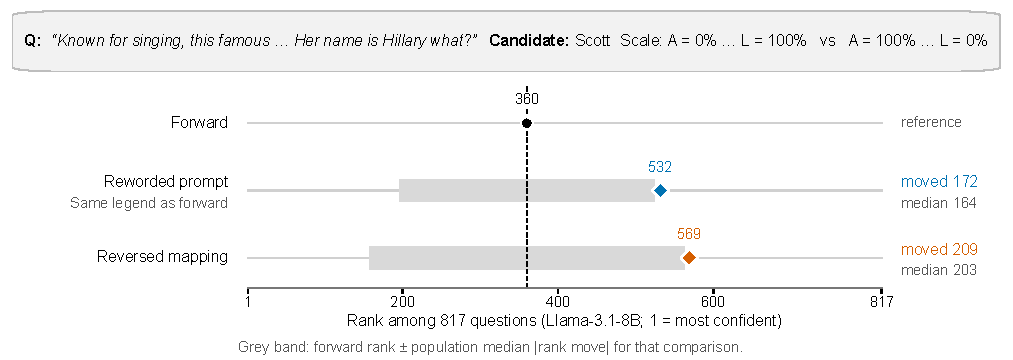
\includegraphics[width=\textwidth]{figs/fig1a.pdf}
\caption{One TruthfulQA item under three elicitations (Llama-3.1-8B). Ranks among all 817
questions (1 $=$ most confident; ties averaged). Grey band: forward rank $\pm$ the population
median absolute rank move for that comparison (164 for rewording, 203 for reversal). The item was
chosen by a pre-specified rule: closest to both population medians in relative distance, ties to
the lowest index.}
\label{fig:legend-item}
\end{figure*}

\paragraph{Setup in full.}
TruthfulQA \citep{lin2022truthfulqa} supplies a correct and an incorrect candidate
answer for each of its 817 questions; a model is shown the question and one candidate
(teacher-forced, no free generation) and asked how confident it is that the candidate is
correct, by choosing a letter A--L. The report $V$ is the expected value of the model's letter
distribution decoded through the legend in force. The three procedures are the forward legend,
the reversed legend (decoded back to the same $0$--$100\%$ scale), and a reworded confidence prompt
under the forward legend. Figures~\ref{fig:legend-item}--\ref{fig:legend-quintile} use the correct
candidate; \expname{Elicitation-Shift} and \expname{Granularity} use one candidate per question chosen by a label-blind hash,
so $Y$ is the correctness of that candidate (about half are correct). Labels do not depend on the
procedure, so $n_{\mathrm{lab}}$ counts labelled questions and every procedure's forecaster is
fitted on the same $n_{\mathrm{lab}}$ questions; a further third of the questions, unlabelled, is
used only to fit the PCA and the groups. Conformal sets are over $Y\in\{0,1\}$; a set of size 2
means abstaining. PopQA is held out in two senses: it is a different dataset, and its questions
are disjoint from those used to train its probe.

\emph{Controlled reporting interventions}: three frozen models
(Llama-3.1-8B, Mistral-7B, Qwen2.5-7B) on TruthfulQA under three elicitations: forward legend,
reversed legend, and a reworded prompt under the forward legend (a fourth, reworded and reversed, is
cached but unused). \emph{Held-out factual QA}: PopQA \citep{mallen2023popqa} (7{,}377 questions) with a linear probe on the
answer's hidden state as the report, and TriviaQA \citep{joshi2017triviaqa} answers of Llama-3.1-8B with trained question-only
and answer-aware correctness reporters. \expname{PopQA-Elicit} repeats the three elicitations, with the
TruthfulQA templates unchanged, on all PopQA questions for the three frozen models, pairing each gold
answer with a distractor that answers the same relation for a different question (type-consistent in
a 256-question audit, where a surface-only classifier could not separate the two: AUROC $0.47$); 188 questions whose distractor matches an accepted alias are
dropped, leaving 7{,}189 (budgets up to about 2{,}400 labels). \emph{Synthetic reliability models}: \expname{Synthetic-Reliability}. Real-data comparisons
use repeated random splits of one pool; because the splits overlap, intervals use the Nadeau--Bengio
correction \citep{nadeau2003inference} (variance factor $1/J+n_{\mathrm{test}}/n_{\mathrm{lab}}$), and the comparison that answers the
registered question (groups vs.\ recalibration, three models $\times$ four budgets) is a pre-declared
family with Holm correction \citep{holm1979simple}. Every logistic forecaster tunes its penalty by inner cross-validation on
the labelled rows; the report's coefficient is penalised a hundred times less than group or feature
coefficients, so tuning does not discard the report.

\paragraph{Ranks.} The report is the expected value of the model's letter distribution, so a
same-prompt redraw moves no rank; the references are a reworded prompt and a shuffled-question null.
Under reversal a typical question moves 203 [184, 222] (Llama), 240 [221, 260] (Mistral) and 190
[173, 208] (Qwen) positions, against 239 [220, 259] under independent rankings and 139--169 under a
reworded prompt; the share of questions that stay in their confidence fifth is $0.240$ [0.208, 0.271],
$0.202$ [0.174, 0.231] and $0.244$ [0.217, 0.278], against $0.284$--$0.337$ under rewording
(Figure~\ref{fig:legend-quintile}). The reports themselves are weak: AUROC for correctness is
$0.54/0.59/0.52$ (Llama; forward/reversed/reworded), $0.40/0.46/0.49$ (Mistral, whose forward report
is anti-informative) and $0.56/0.46/0.60$ (Qwen).

\begin{figure*}[t]
\centering
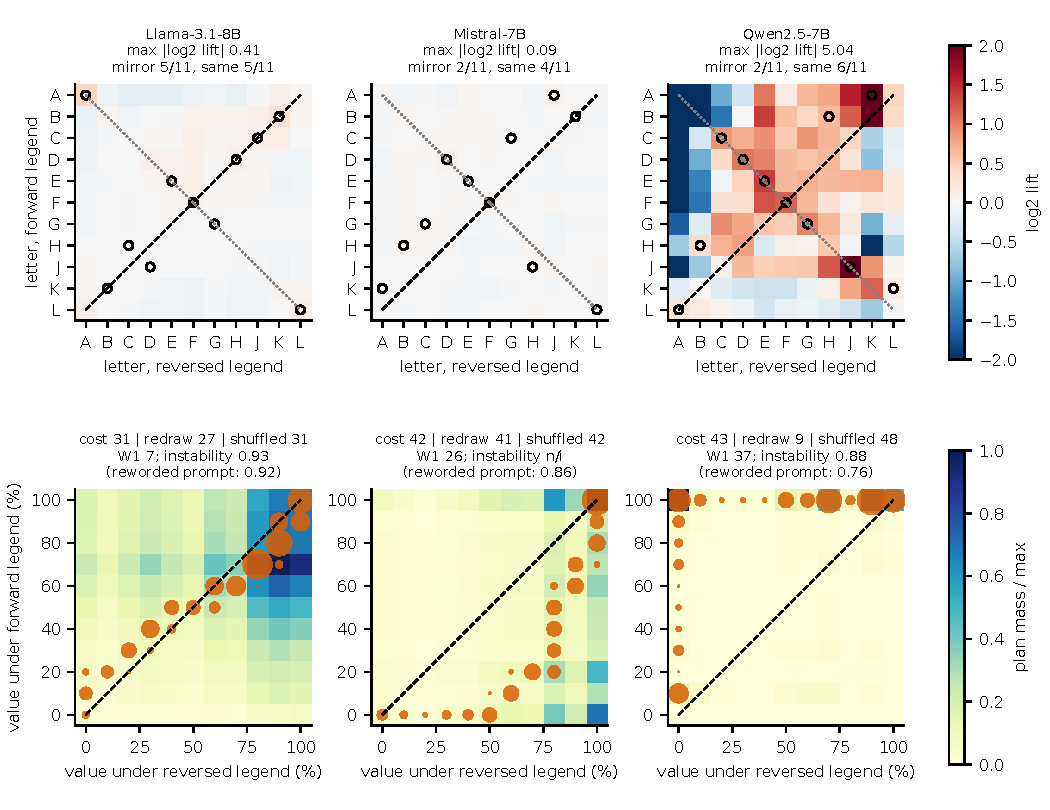
\includegraphics[width=\textwidth]{figs/fig_transport.pdf}
\caption{Forward-to-reversed transport plans (817 TruthfulQA questions, both candidates; letters A--L
skip I). Top: $\log_2$ lift of letter co-occurrence over independence; circles: Hungarian alignment on
lift; dashed: \emph{mirror} (the letter with the same value under the reversed legend, i.e.\ the legend
is read), dotted: \emph{same letter} (the legend is ignored). Bottom: realised plan on the value scale;
orange: optimal monotone ($W_1$) plan between the two marginals, i.e.\ what recalibrating the report
could achieve. Titles: realised cost against an independent redraw under the forward legend (a stable
but noisy report) and against shuffled questions; instability $=$ (realised $-$ redraw)/(shuffled $-$
redraw).}
\label{fig:transport}
\end{figure*}

\paragraph{Transport plans.} Because the forward and reversed prompts are
separate calls, the joint law of the two reports for a random question is the average over
questions of the product of their letter distributions: an empirical transport plan from forward
to reversed reports (Figure~\ref{fig:transport}). Measured on the value scale against two
references --- an independent redraw under the forward legend (a stable but noisy report) and
shuffled questions --- the realised cost sits at $85$--$93\%$ of the way from redraw to shuffle
for all three models (reworded prompt: $76$--$92\%$); for Mistral under reversal the shuffled and redraw costs differ by only $0.5$ points, so its index is not interpretable. For Llama and Mistral the letter plan has
almost no lift over independence (max $|\log_2 \mathrm{lift}|$ of $0.41$ and $0.09$), so no letter alignment is
identified: the reversed report says almost nothing question-specific about the forward one. Qwen
shows strong same-letter lift (max $5.0$): it partly ignores the legend, which appears on the value
scale as a flip. The optimal monotone plan separates what recalibration can repair: most of
Qwen's cost is a level shift ($W_1=37$ of $43$), most of Llama's is question-level reshuffling
($W_1=7$ of $31$) that no recalibration of the report can undo --- the case in which structure
from a frozen representation (\expname{Granularity}) has room to help.

\paragraph{Quintile transitions.}
\begin{figure*}[t]
\centering
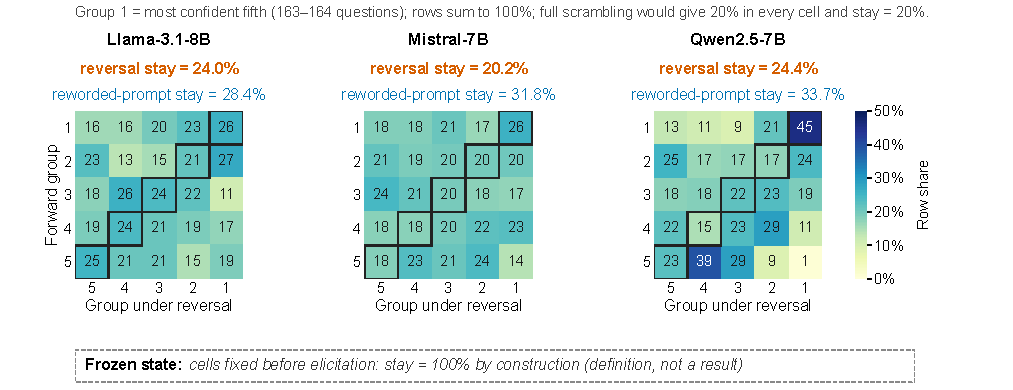
\includegraphics[width=\textwidth]{figs/fig4_quintile_reversal.pdf}
\caption{Where each fifth of questions lands under legend reversal (rows: forward fifth,
1 $=$ most confident; columns: fifth under reversal; rows sum to 100\%; full scrambling gives
20\% everywhere). Stay share (mean diagonal) under reversal is near the 20\% null for all three
models and below the stay share under prompt rewording. Qwen partly preserves its extremes
(45\% of its most confident fifth stays there). A binning fixed before elicitation stays put by
construction; that is a definition, not a result. What matters for coverage is
Section~\ref{sec:experiments} (\expname{Elicitation-Shift}).}
\label{fig:legend-quintile}
\end{figure*}

\paragraph{Per-split coverage.}
Per split, the 10th--90th percentiles of coverage are $0.87$--$0.94$ for every same-elicitation arm,
$0.50$--$0.59$ and $0.56$--$0.66$ for Mistral under reversal and rewording, and $0.95$--$0.99$ for Qwen
under rewording. On TruthfulQA only Mistral under-covers and Llama and Qwen become conservative; on
PopQA Llama under-covers too under reversal ($0.76$), while Qwen again becomes conservative.

\paragraph{Granularity figure.}
\begin{figure*}[t]
\centering
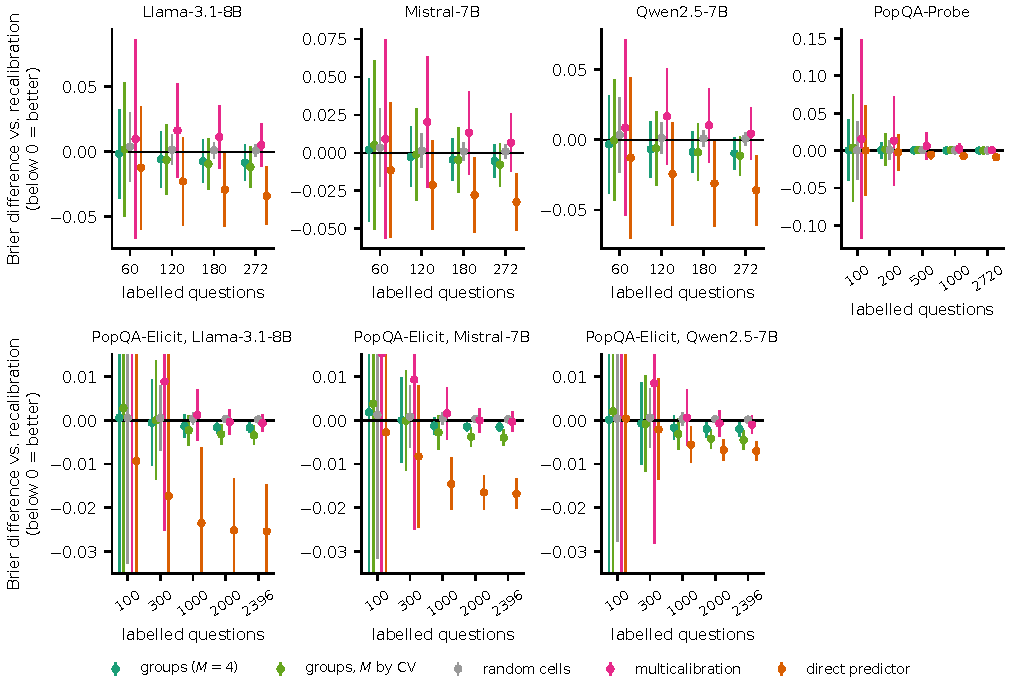
\includegraphics[width=\textwidth]{figs/fig_e5.pdf}
\caption{Brier difference against procedure-specific recalibration R (below zero: better), averaged over
procedures, with Nadeau--Bengio-corrected 95\% intervals. Top: TruthfulQA (three models, 200 random
splits) and \expname{PopQA-Probe} (probe report, one procedure, 100 splits). Bottom: \expname{PopQA-Elicit} (three
models, three procedures, 100 splits); the vertical axis is zoomed, so intervals at 100--300 labels run
beyond it. Groups: farthest-first cells on 16 PCA dimensions of the frozen hidden state.}
\label{fig:e5}
\end{figure*}

\paragraph{Granularity on TruthfulQA and PopQA-Probe, in full.}
On TruthfulQA the reports are nearly uninformative: recalibrated, they score within $0.003$ Brier of
the base rate. Groups improve on them in 84--95\% of splits at 272 labels ($-0.005$ to $-0.010$ Brier,
a Brier skill over the base rate of 3--5\%), but no test in the pre-declared family survives Holm
correction (smallest one-sided $p=0.044$, Qwen at 272 labels), and at 60 labels groups are as likely to
hurt as to help. Groups from the representation beat random groups of the same number in 85--96\% of
splits (intervals include zero); TruthfulQA's own categories do not help. The number of groups chosen by
cross-validation spreads over 4, 8 and 16 at 272 labels, and one group stops being chosen
($P(M=1)$ falls from $0.23$--$0.32$ at 60 labels to $\le0.01$): the best granularity grows only in this
weak sense. Multicalibration with a holdout never beats the recalibration it starts from: the holdout
costs more than the patches gain at these budgets. Group offsets shared across the three procedures
differ from per-procedure groups by at most $0.0012$ Brier at every budget, but a pre-specified
equivalence test with margin $\pm0.002$ does not establish equivalence (90\% corrected intervals at 272
labels, e.g.\ $[-0.0019,0.0021]$ for Llama). The direct predictor D, on the same representation,
beats R by $0.032$--$0.036$ at 272 labels (Brier skill 14--15\%; intervals exclude zero from 180 labels)
and beats groups ($M=4$) by $0.026$--$0.027$; it is ahead of R in 90\% of splits even at 60 labels. On PopQA,
whose probe report is miscalibrated but discriminative (AUROC $0.73$; skill $0.16$ after
recalibration), groups show no gain at any budget ($|$G$_4-$R$|\le0.0005$) while D helps from 1{,}000 labels (corrected
interval; it is ahead in every split from 500).

\paragraph{Binned calibration error.}
Binned calibration error tells a different and less reliable story:
at 272 labels the class-wise calibration error (SCE, calibration-toolbox) of groups and of the direct
predictor is higher than recalibration's ($0.066$--$0.072$ and $0.087$--$0.090$ against $0.048$--$0.054$;
every corrected interval includes zero), and the constant base rate scores best ($0.035$). On about 272
test questions with 15 bins, a forecast that varies more spreads over more, sparser bins and pays a
larger upward bias, and a constant forecast is calibrated without discriminating; we therefore rank
forecasters by Brier score and report binned errors as diagnostics only.
The PopQA contrast changes the dataset, the report and the single procedure at once, and its probe is
built on the representation the groups use, so it is one observation rather than a de-confounded
effect; \expname{Synthetic-Reliability} isolates the factors.

\paragraph{\expname{Synthetic-Reliability}: synthetic reliability models (post hoc).} A latent signal $u$ and a group
effect $\beta$ determine $\P(Y=1)=\sigma(\beta+u)$; reports under three procedures are noisy,
level-shifted views of $u$ with informativeness $\kappa$; $\beta$ varies either across 32 clusters in
four dimensions (not representable by a linear function) or linearly in the features, with spread
$\tau$. Groups (farthest-first, $M$ by inner cross-validation), recalibration and the direct predictor
are fitted on $n_{\mathrm{lab}}$ labels (Figure~\ref{fig:synth}; 30 independent seeds per
configuration). Without a group effect ($\tau=0$) groups lose to recalibration at every budget: pure
estimation cost. With a group effect they win only once labels suffice (linear structure: $\tau\ge1$
from 120 labels; cluster structure: $\tau=2$ at 480 labels). Report informativeness $\kappa$ barely
moves either comparison: the lines for $\kappa\in\{0,0.5,1,2\}$ overlap in every panel. Against the
direct predictor groups never win; they tie at best, including when reliability is a non-linear
function of the features. A first version placed 8 clusters in 8 dimensions, which is secretly linear;
it gave the same answer (Appendix~\ref{app:protocol}).

\paragraph{\expname{Real-Geometry}: known reliability on real representations.} The synthetic
features above are Gaussian. To keep the geometry real while knowing the truth, we use the 7{,}377
PopQA hidden states of Llama-3.1-8B as features and simulate only the outcome:
$\P(Y=1)=\sigma(\beta(x)+u)$, with $\beta$ constant on 32 $k$-means clusters of a 64-dimensional PCA
(which the methods, seeing 16 dimensions, cannot represent exactly) or linear in the features, spread
$\tau\in\{0,0.5,1,2\}$, and reports as in \expname{Synthetic-Reliability}. Because $\eta=\P(Y=1\mid x,u)$ is known we
score the pointwise error $\E(\hat f-\eta)^2$ directly (20 seeds per configuration, budgets 100 to
2{,}000). The pattern is the synthetic one; differences are in units of $10^{-3}$. Without a group effect
groups cost $+2.5$ to $+5.9$ at 100 labels, shrinking to $+0.1$ to $+0.3$ at 2{,}000. With one they win
once labels suffice: cluster structure, $\tau=1$ from 300 labels ($-3$ to $-10$) and $\tau=2$ from 300
($-17$ to $-31$); linear structure, $\tau\ge1$ from 100 labels ($-6$ to $-68$). The direct predictor is ahead of
groups wherever there is structure and at least 300 labels, cluster structure included ($+0.3$ to $+25$; the interval excludes zero in 49 of 54 such configurations),
and loses to them only when there is nothing to find ($\tau=0$, $n\ge1{,}000$: $-0.9$ to $-1.6$, intervals
below zero), where cross-validation picks $1.5$--$3.5$ groups on average, close to recalibration, while D pays for 16 null coefficients. Report informativeness again changes
nothing.

\begin{figure*}[t]
\centering
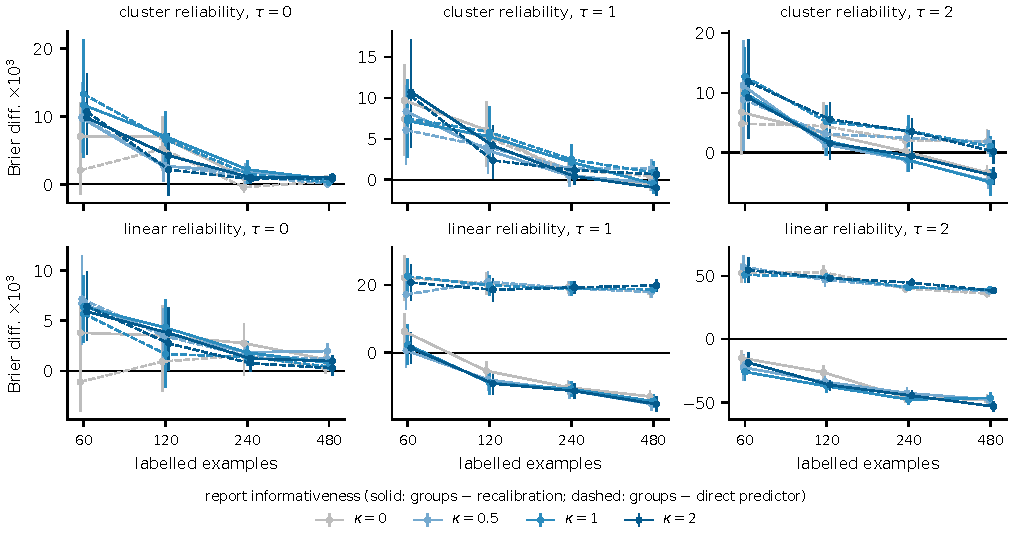
\includegraphics[width=\textwidth]{figs/fig_synth.pdf}
\caption{Synthetic reliability models. Brier difference ($\times10^3$) of groups minus recalibration
(solid) and groups minus the direct predictor (dashed), against labelled examples, for report
informativeness $\kappa$ (colour) and between-group spread $\tau$ (columns); 95\% intervals over 30
independent seeds per configuration. Top: reliability varies across 32 clusters in four dimensions;
bottom: linearly.}
\label{fig:synth}
\end{figure*}

\paragraph{Conformal sets (post hoc).} With forecasters fitted on half of the labels and
thresholds on the other half, every forecaster is valid. With one threshold for all questions, the
group forecaster's sets are $0.03$--$0.07$ labels smaller than recalibration's at
$\alpha\in\{0.1,0.2,0.3\}$ (e.g.\ $1.74$ against $1.80$ for Llama at $\alpha=0.1$), but every corrected
interval includes zero; the direct predictor's sets are smaller still ($1.62$--$1.65$, with
$0.35$--$0.38$ singletons against $0.20$--$0.22$). With one threshold per group, the half-split leaves
some groups below the calibration floor (15\% of test mass receives the full set), so group-Mondrian
sets over-cover ($0.92$) and are no smaller than recalibration's: per-group guarantees cost efficiency
at these budgets. A Brier gain of $0.008$ moves few forecasts across a threshold, so the groups' gain in
correctness prediction barely reaches the sets; the direct predictor's larger gain does. On PopQA all
forecasters give sets of the same size.

\section{Transport across procedures: full results and controls}
\label{app:transport}
This appendix collects the transport results summarised in Section~\ref{sec:exp-transport}. Transport is
presented as a repair that is checked empirically: the only guarantee is the label-loss lower bound of
Proposition~\ref{prop:transport}(a), and the exact transfer of (b) holds only for the population map
under an exactly monotone change.

\paragraph{\expname{Label-Free-Transfer}: carrying a calibration across procedures without labels.} (Criteria fixed in a
dated note before the run; the experiment was designed after the coverage breaks of
Section~\ref{sec:exp-break} had been seen and after the reversed trained reporter was known to be
anti-correlated with the original, so it is not a test of a prior prediction.) A forecaster and
conformal thresholds are fitted under procedure A with labels; deployment is under B. Two label-free
maps carry $V_B$ back to A's scale, both fitted on the unlabelled third of the questions, which are
elicited under both procedures: the \emph{quantile map} $F_A^{-1}\circ F_B$, the monotone
optimal-transport map between the two marginals (unpaired, increasing), and \emph{paired isotonic}
regression of $V_A$ on $V_B$ over the same questions, with its direction (increasing or decreasing)
chosen by fit (Proposition~\ref{prop:transport}). Under A, Platt scaling and the conformal thresholds are fitted on disjoint halves of the labelled third
(the honest split of Section~\ref{sec:setup}; an earlier run fitted both on the same half and was
replaced). The labelled reference recalibrates under B with $k$ labelled questions, half to fit Platt
scaling and half to set the threshold. Frozen models: 500 random thirds; trained TriviaQA reporters: one
split. Same-procedure coverage is $0.919$--$0.922$ on TruthfulQA, slightly conservative because each
threshold now rests on about 34 points per group.
Paired isotonic regression repaired the one change that was monotone question by question: it found,
without labels, that the reversed question-only reporter runs backwards, and restored coverage ($0.206\to
0.910$, against $0.909$ under the original procedure), set size and Brier score ($0.1232$ against $0.1228$;
one split), better than recalibrating on $60{+}60$ labels ($0.128$). The quantile map cannot represent a
decreasing change and fails there ($0.780$). On the frozen models, where questions are reshuffled, paired
isotonic regression regresses towards the mean and becomes conservative with near-full sets ($0.94$--$0.99$,
sizes $1.88$--$1.99$), while the quantile map keeps A's set size and moves coverage most of the way back
(Mistral from $0.60$--$0.63$ to $0.89$--$0.90$). Its near-exact matches for Llama and Qwen come where the
forecasts are close to the base rate (Brier $\approx0.25$, sets $\approx1.8$ of 2 labels), so they say
little about informative reports. Mapping within frozen groups changes coverage by at most $0.016$.
The two-sided crossing mass of Proposition~\ref{prop:transport}(a) is $0.16$--$0.32$ on the frozen models
and says little. The one-sided label-loss mass is more useful but must carry its estimation error: for
paired isotonic regression it is $0.013$ for the question-only reporter, so with $m=10{,}647$ test
questions and $\delta=0.05$ (Hoeffding term $0.012$) coverage under B is at most $0.025$ below A's, with
set sizes unchanged; on Llama and Mistral it is $0.006$--$0.027$, but only because the map widens sets
to near-full, and with about 272 test questions per split the Hoeffding term is $0.074$. For the quantile
map, which keeps set size, it is $0.10$--$0.17$, which certifies little. Full results, including Brier
scores, split quantiles, label-loss masses and per-group gaps, are in Appendix~\ref{app:e8}.

\paragraph{Transfer on PopQA.} On \expname{PopQA-Elicit} (100 random thirds of 7{,}189
questions) the same forecaster, unmapped, falls to $0.53$--$0.60$ under reversal for all three models
(and to $0.57$ for Mistral under rewording). The quantile map moves it to $0.84$--$0.95$: close for Qwen
($0.896$, $0.894$) and Llama under rewording ($0.902$), but too high for Llama under reversal ($0.951$)
and too low for Mistral ($0.842$, $0.874$). Paired isotonic regression found that Mistral's reversal
runs backwards (decreasing in every split), but its sets are near-full ($0.965$ coverage, size $1.92$);
for Llama it returns the full set, and for Qwen it falls to $0.876$. Recalibrating on $60{+}60$ labels gives
$0.90$ on average everywhere, but judged by the same standard as the maps it is not tighter split by split
(10--90\% range $0.84$--$0.95$, against $0.88$--$0.91$ for the quantile map on Qwen). Because the reversed
legend is more informative than the forward one for Llama and Mistral on PopQA, recalibrating under it also
beats carrying the old calibration over (Brier $0.214$ and $0.226$ against $0.245$ and $0.251$). With
informative reports and a larger pool, then, label-free maps repair most of the break but none is
reliably exact. The label-loss mass (Hoeffding term $0.025$ at $\delta=0.05$ for 2{,}396 test questions)
certifies a small loss only where paired isotonic regression widens sets ($0.003$--$0.006$ for Llama with
near-full sets, $0.06$--$0.07$ for Mistral); for the quantile map it is $0.15$--$0.26$.

\paragraph{Calibration of the carried forecast.} Coverage
is a property of sets; we also scored the carried forecasts with the class-wise calibration error
(SCE, 15 equal-width bins; for two classes it equals the binary ECE of the forecast) from the
calibration-toolbox package \citep{pearce2026calibrationtoolbox}, pooling test predictions over 50
splits (Figure~\ref{fig:reliability}, Appendix~\ref{app:e8}). Without a map the forecast is badly
miscalibrated (SCE $0.28$--$0.29$ for Mistral, $0.73$ for the reversed question-only reporter, against
$0.016$--$0.020$ under the original procedure). Paired isotonic regression has the lower SCE on TruthfulQA
and TriviaQA ($0.035$--$0.040$ for Mistral, $0.016$ for the question-only reporter), the quantile map
$0.051$--$0.070$ for Mistral and $0.26$ for the decreasing change it cannot represent; on PopQA the two are
close ($0.011$ and $0.014$ for Mistral under reversal). Binned error is a diagnostic, not a ranking: a
constant forecast at the test base rate scores $0.000$ in every panel, and for Mistral paired isotonic
regression attains its low error by compressing forecasts into $[0.37,0.61]$, which is also why its sets
widen, while the quantile map keeps the spread and the set size. Throughout, we rank forecasters by Brier
score and report binned errors only alongside it.

\paragraph{\expname{Failure-Modes}: what breaks which method.} Under one protocol we
apply to every method (bins of the report, representation groups with model~\eqref{eq:forecaster},
multicalibration, the direct predictor with and without the report) the shifts that could break it: a
monotone level change, a reversal, the real rewording, and a permutation of the reports across a share
$\rho$ of questions, each raw, after the quantile map and after paired isotonic regression (100 splits
per model; criteria in a dated note). Both pre-set checks pass for all three models: with no shift the
maps move coverage by less than $0.005$, and after a monotone level change the quantile map restores
coverage within $0.01$. Three findings. (i) The direct predictor that uses only the representation is
invariant to the elicitation by construction and covers $0.904$--$0.908$ under every shift, with sets of
$1.61$--$1.63$ against $1.75$--$1.82$ for bins, groups and multicalibration; the direct predictor that
also reads the report has sets as small ($1.58$--$1.62$) but inherits the report's shifts. The
invariant predictor is not the best calibrated (per-split SCE $0.10$--$0.11$ against $0.05$--$0.07$ for
recalibrated bins), so its advantage is in sets and robustness rather than in calibration: when the
representation is available, not reading the report is the robust choice. (ii) The real rewording
breaks every report-based method for Mistral, groups and multicalibration included (coverage
$0.55$--$0.66$); the quantile map restores all of them to $0.87$--$0.89$. Groups do not protect against
an elicitation change, because the report enters their forecast. (iii) Paired isotonic regression
fails in a direction that depends on the kind of reordering: conservative under additive noise
(\expname{Controlled-Shifts}), but under-covering when reports are fully permuted for Llama and Qwen
($0.87$, $0.86$). Report bins also move: under rewording 43--68\% of test mass changes bin, so per-bin
guarantees attach to different questions than at calibration, while representation groups do not move.
On \expname{PopQA-Elicit} (50 splits) both
pre-set checks pass again and the state-only direct predictor is again invariant ($0.899$--$0.903$), but
the reports are informative there, so for Qwen its sets are larger than those of report-based methods
($1.74$ against $1.53$--$1.62$): not reading the report buys robustness at a cost in efficiency once the
report carries information. Rewording now hurts representation groups and multicalibration more than
report bins (Llama: $0.83$--$0.84$ against $0.91$; Qwen: $0.72$--$0.73$ against $0.92$), because their forecast
reads the report through coefficients fitted under the old wording; the quantile map does not repair
them for Llama ($0.84$) and only partly for Qwen ($0.86$). Qwen's forward reports put 63\% of their mass beyond $0.02$ or $0.98$ (15\% ties), so its
quantile maps are degenerate and fail under reversal ($0.55$--$0.73$).

\paragraph{Labelled transfer.} Reusing group offsets fitted under one procedure and refitting only the
report slope and intercept on $k$ labels under the new one was numerically unstable at small $k$
(split-level Brier scores up to $0.58$); we do not draw conclusions from it.

\paragraph{\expname{Controlled-Shifts}: the transport proposition on real reports.} We build
procedure B from real procedure-A reports, $\operatorname{logit}V_B=s\operatorname{logit}V_A+b+\sigma\,
\mathrm{sd}(\operatorname{logit}V_A)\,\varepsilon$, with $s=\pm1$, $b\in\{0,1\}$ and question-level noise
$\sigma\in[0,2]$, on the three frozen models (100 splits) and the TriviaQA answer-aware reporter. At
$\sigma=0$ the predictions of Proposition~\ref{prop:transport} are mathematical, so this part checks the
implementation and the finite-sample behaviour of the fitted maps; all three hold on all four datasets,
as fixed before the run. Paired isotonic regression recovers A's coverage for both signs (mean per-split
$|\Delta\text{coverage}|\le0.0004$), and the quantile map does so only for $s=+1$ ($\le0.003$); under
reversal it misses by $0.03$--$0.07$ per split on the frozen models and $0.22$ on TriviaQA (mean coverage
$0.84$--$0.90$ and $0.69$, against $0.90$--$0.91$; for Llama and Qwen the per-split errors largely average
out). The crossing mass is near zero at $\sigma=0$ and grows with $\sigma$; the bound
$|\Delta\text{coverage}|\le$ crossing mass holds in every split, as it must, because both are computed on
the same test questions. The informative part is $\sigma>0$: at $\sigma=2$ the quantile map keeps A's set
size and stays at $0.89$--$0.91$ on the frozen models for an increasing change, but falls to $0.86$ for
Mistral under reversal and to $0.80$ and $0.71$ for the TriviaQA reporter, while paired isotonic regression
regresses towards the mean and becomes conservative ($0.97$--$0.98$ with sets of $1.95$--$1.96$ on the frozen
models, $0.92$ with sets of $1.39$ on TriviaQA).

\paragraph{Controls and map variants.} These arms were added after an external design review, with
criteria fixed in a dated note before the run; they change no number reported above.
(i)~\emph{Oracles.} In \expname{Controlled-Shifts} the true noiseless inverse of the synthetic change reproduces
A's coverage exactly at $\sigma=0$ on all four datasets (the identity control is the no-shift arm of
\expname{Failure-Modes}, which moves coverage by less than $0.005$). Under noise the oracle does worse than the
fitted maps ($|\Delta\text{coverage}|$ $0.06$--$0.08$ at $\sigma=1$, against $0.02$ for the quantile map under
an increasing change on the frozen models), because noise changes the law of $V_B$: the useful target is
$\E[V_A\mid V_B]$, which isotonic regression estimates, not $g^{-1}$.
(ii)~\emph{Direction.} An isotonic map forced in the wrong direction collapses to a constant forecast:
for the reversed question-only reporter the increasing fit gives coverage $0.81$ with singleton sets
and the decreasing fit $0.910$, and in \expname{Controlled-Shifts} a wrong-direction fit misses by $0.09$--$0.10$ at
$\sigma=0$. On the frozen models both directions give near-full sets under the real reversal (coverage
$0.94$--$1.00$, sizes $1.88$--$2.00$), so reversing the legend does not flip the decoded report
monotonically and neither fixed direction repairs it; on PopQA a decreasing fit gives $0.68$ for Qwen.
(iii)~\emph{Mid-rank map.} A quantile map whose CDFs use mid-ranks, both stored from the transport fold
and frozen, agrees with the map used above within $0.001$ coverage everywhere, including the TriviaQA
reporters, whose reports have 5--32\% ties, and Qwen's forward PopQA report with 15\% ties; with atoms
no deterministic map matches the two marginals exactly.
(iv)~\emph{Permutation.} Permuting reports across a share $\rho$ of questions keeps the marginal, so the
quantile map cannot see it. At $\rho=1$ paired isotonic regression ranges from $0.79$ to $1.00$ across the
three models and two datasets: it under-covers for Llama and Qwen on TruthfulQA ($0.87$, $0.86$) and for
Mistral on PopQA ($0.79$), and over-covers in the other three (\expname{Failure-Modes}).
(v)~\emph{Per-group coverage.} The worst of the four frozen groups is below the target even without a shift
(the A$\to$A arm's worst group is $0.02$--$0.04$ short), so gaps are reported net of that baseline
(Appendix~\ref{app:e8}). Net, no arm keeps every group: recalibrating on $60{+}60$ labels, which uses one
threshold for all groups, leaves the worst group $0.08$--$0.15$ short on TruthfulQA and up to $0.06$ short on
PopQA; the quantile map leaves it up to $0.05$ short on TruthfulQA and up to $0.18$ short on PopQA; and
paired isotonic regression keeps every group only where it widens sets to near-full, falling $0.19$ short for
Qwen on PopQA. Per-group guarantees after a change of procedure therefore need per-group recalibration
under the new procedure, which our label budgets do not support.

\section{Post-hoc analyses added after the experiment lock}
\label{app:postlock}
These
two analyses were added on 5 October, after the experiments had been locked, following an external
suggestion; their design was fixed in a dated note before they ran, they reuse the cached states and splits
above, and they are descriptive and outside the pre-declared Holm family.

\paragraph{Partition efficiency with a fixed score.} Each split fits one correctness model on half of the
labelled third (Platt on the report, R, or the direct predictor, D) and holds it fixed; only the partition and its
per-cell thresholds, set on the other half with a floor of 20, change (100 splits, averaged over procedures).
\begin{table*}[t]
\caption{Post-hoc partition-efficiency check: one correctness model per split is held fixed (R or D) and only the partition changes; mean set size, fallback mass (test mass in cells below the floor) and worst-cell coverage, ranges over the three models, 100 splits.}
\centering\small
\begin{adjustbox}{max width=\textwidth}
\begin{tabular}{llcccc}
\toprule
data (calibration points) & partition & set size (R) & set size (D) & fallback mass & worst cell coverage (R)\\
\midrule
TruthfulQA (136) & one cell & 1.78--1.80 & 1.62--1.64 & 0.00 & 0.90--0.91\\
 & report bins, $M=4$ / 8 & 1.80--1.81 / 1.94--1.95 & 1.64--1.67 / 1.89--1.90 & 0.01 / 0.68--0.69 & 0.85 / 0.87--0.88\\
 & representation cells, $M=4$ / 8 & 1.80--1.83 / 1.85--1.89 & 1.69--1.73 / 1.77--1.83 & 0.15 / 0.35--0.41 & 0.88--0.90 / 0.88--0.89\\
PopQA (1{,}198) & one cell & 1.60--1.68 & 1.55--1.59 & 0.00 & 0.90\\
 & report bins, $M=4$ / 8 & 1.61--1.69 / 1.64--1.71 & 1.56--1.59 / 1.56--1.60 & 0.00 & 0.88 / 0.86\\
 & representation cells, $M=4$ / 8 & 1.59--1.68 / 1.59--1.68 & 1.55--1.59 / 1.56--1.59 & 0.00 & 0.87--0.88 / 0.85\\
\bottomrule
\end{tabular}
\end{adjustbox}
\end{table*}
Coverage is at least $0.90$ for every arm. On PopQA, representation cells change the mean set size by at
most $0.006$ against one cell; report bins enlarge it slightly. On TruthfulQA, every partition finer than one
cell enlarges sets, because cells fall below the floor and return the full set. The score matters far more
than the partition: replacing R by D shrinks sets by $0.12$ (PopQA, Llama) and $0.16$ (TruthfulQA). Worst-cell
coverage falls with $M$ because the minimum over more, smaller cells is noisier; it is not a per-cell guarantee
failure. At these budgets, then, frozen cells do not make conformal sets more efficient for a fixed score.

\paragraph{Correctness-probe baselines.} On the same splits and label budgets as \expname{Granularity}, we compare
recalibrating the report (R) with a probe on the full candidate-conditioned hidden state, specified as in
\citet{moreno2025correctness} (standardised features, logistic regression with default penalty and balanced class
weights; P-full), a tuned, unweighted probe on 16 PCA dimensions (P16), the report combined with a cross-fitted P16
score (V$+$P), groups (G$_4$) and the direct predictor (D). Labels spent on a probe count against the same budget.
Brier differences against R at the largest budget ($\times10^3$, corrected 95\% intervals):
\begin{table*}[t]
\caption{Post-hoc correctness-probe baselines: Brier difference against recalibrating the report ($\times10^3$; below zero: better) at the largest budget, with Nadeau--Bengio-corrected 95\% intervals for P-full.}
\centering\small
\begin{adjustbox}{max width=\textwidth}
\begin{tabular}{llccccc}
\toprule
data & model & P-full & P16 & V$+$P & G$_4$ & D\\
\midrule
TruthfulQA, 272 & Llama & $-44.7$ [$-83.3$, $-6.2$] & $-30.2$ & $-32.7$ & $-8.8$ & $-34.2$\\
 & Mistral & $-42.1$ [$-75.8$, $-8.3$] & $-31.2$ & $-31.0$ & $-5.2$ & $-32.1$\\
 & Qwen & $-57.1$ [$-95.4$, $-18.8$] & $-31.4$ & $-33.6$ & $-9.8$ & $-36.3$\\
PopQA, 2{,}396 & Llama & $+74.2$ [$56.8$, $91.5$] & $-16.8$ & $-23.6$ & $-1.7$ & $-25.4$\\
 & Mistral & $+69.3$ [$53.3$, $85.3$] & $+1.9$ & $-12.6$ & $-1.5$ & $-16.8$\\
 & Qwen & $+127.0$ [$109.7$, $144.2$] & $+25.7$ & $-0.8$ & $-2.0$ & $-7.0$\\
\bottomrule
\end{tabular}
\end{adjustbox}
\end{table*}
On TruthfulQA the full-state probe is the best forecaster (AUROC $0.81$--$0.83$, against $0.70$--$0.72$ for D), so
the 16-dimensional direct predictor of the main text understates how much a learned predictor on the
representation can gain. On PopQA the same probe is badly miscalibrated (Brier $0.30$--$0.34$): balanced class
weights and an untuned penalty on 4{,}096 dimensions overfit even at 2{,}396 labels. The probe alone on 16
dimensions is mixed; combined with the report it is close to D. In every setting, groups gain less than every
representation-based predictor except the miscalibrated full probe on PopQA.

\section{Additional results}
\label{app:extra}
\subsection{\expname{Known-Law}: known conditional law}
\label{app:x1}
\paragraph{\expname{Known-Law}: known conditional CDF.}
$X\sim\mathrm{U}[0,1]^d$, $S=(0.4+1.6\,\bar X)\,U$, so $F_x$ is known and $R_{\mathrm{pt}}$,
its decomposition and all cell functionals are computed exactly on 12{,}000 test points.
$k$-means exemplars snapped to $\Dfit$ ($n_{\mathrm{fit}}=4000$), $\alpha=0.1$, floor 20,
19 values of $M$ from 1 to 190 (ratio $\approx1.3$), 8 values of $n_{\mathrm{cal}}$ from 300 to
8000, 20 seeds, 1000 whole-seed bootstrap resamples. $M^\star$ is the vertex of a local
quadratic in $\log M$.

\emph{Results, $d=1$, $k$-means arm}. The decomposition is exact (residual $\le10^{-12}$). The
cell-level term matches the Beta expectation of Corollary~\ref{cor:B0} (seed-mean
difference $1.4\times10^{-5}$, SE $2.9\times10^{-5}$), and cell MSCE is minimised at $M=1$ for
every $n_{\mathrm{cal}}$, as are concentrated undercoverage under the efficiency constraint.
The pointwise gap has an interior minimiser at every $n_{\mathrm{cal}}$ (99.8\% of bootstrap
replicates), with $M^\star$ rising from $8.4$ to $35.2$. Its log-log slope is $0.417$
$[0.395,0.441]$. The quantisation term decays as $M^{-\hat a}$ with $\hat a=1.82$
$[1.79,1.84]$, predicting a slope $1/(\hat a+1)=0.355$; the difference has CI
$[0.042,0.086]$, inside the pre-set $\pm0.10$ margin.
Descriptively, the slope interval excludes the asymptotic $1/3$ and $\hat a$ is below $2$: the
grid is pre-asymptotic. The floor is inactive at the discrete $M^\star$ for every
$n_{\mathrm{cal}}$, and $R_{\mathrm{pt}}(M^\star)$ is at most $0.47$ of the floor ceiling
$(1-t)^2$; dropping $n_{\mathrm{cal}}=300$, where floor activity begins one grid step past
$M^\star$, leaves the result inside the margin (difference CI $[-0.001,0.061]$; post hoc).

\emph{Farthest-first arm (the arm Lemma~\ref{lem:diam} covers)}. Interior optimum (rate
$1.0$), B0 and the decomposition hold at $d=1$ and $d=2$; $M^\star$ rises from $9.1$ to $37.2$
($d=1$) and from $10.3$ to $87.2$ ($d=2$). The mechanism check fails narrowly at $d=1$ (difference
CI $[0.050,0.102]$ against the $\pm0.10$ margin) and clearly at $d=2$ ($[0.071,0.133]$); in both
the slope exceeds $1/(\hat a+1)$, which Remark~\ref{rem:drift} explains post hoc. The $k$-means results
below are a secondary arm, not covered by the lemma.

\emph{Results, $d=2$, $k$-means} (gate FAIL). Interior optimum, B0 and the decomposition checks all hold
($M^\star$ from $10.0$ to $83.1$). The slope is $0.654$ $[0.626,0.685]$ against a predicted
$0.565$ ($\hat a=0.77$); the difference CI $[0.069,0.122]$ exceeds the margin. The equivalence interval is narrow (width $0.053$), so this is a miss, not a lack of power.
Two post-hoc diagnostics locate it. The calibration term behaves as assumed: regressing on
$\log M$ and $\log n_{\mathrm{cal}}$ gives exponents $0.94$ and $-0.96$. The floor is active at
$M^\star$ for $n_{\mathrm{cal}}\le800$, but dropping those points does not restore agreement
(difference CI $[0.007,0.147]$). What fails is the pooled power law for the quantisation term:
its local exponent rises from $0.61$ ($M\approx10$) to $1.0$ ($M\approx130$), and
Remark~\ref{rem:drift} shows a rising exponent steepens the $M^\star$ slope. A post-hoc fit of
that one-parameter correction ($a\approx0.75$, $a'\approx0.17$, read off the same curves) gives
$\approx0.65$ against the observed $0.654$; it is an explanation, not a test.
\subsection{\expname{Answerability}: which stage licenses which bins}
\label{app:x4}
\paragraph{\expname{Answerability}: which stage licenses which bins.}
DGP of Section~\ref{sec:validity}: latent answerability $a(X)$, two independent decodes, the
shown answer's score $S=YU+(1-Y)(1+U)$; $V_{\mathrm{pre}}$, $V_{\mathrm{post}}$ (same decode
as the score) and $V_{\mathrm{post}}'$ (a fresh decode) are each cut into five $\Dfit$-quantile
bins. $n_{\mathrm{fit}}=n_{\mathrm{cal}}=2000$, $n_{\mathrm{test}}=20{,}000$, 50 seeds, six
values of $p=\P(Y=1)$ from $0.24$ to $0.99$. 

\begin{table*}[t]
\caption{X4: coverage on the full test stream by stratifier and answerability rate $p$ (50 seeds; worst bin is the seed mean of the worst bin).}
\centering\small
\begin{adjustbox}{max width=\textwidth}
\begin{tabular}{lcccccc}
\toprule
$p$ & 0.24 & 0.39 & 0.50 & 0.67 & 0.85 & 0.99\\
\midrule
marginal (stage 0)              & .901 & .900 & .900 & .899 & .900 & .901\\
$V_{\mathrm{pre}}$ bins (stage 0)  & .902 & .901 & .900 & .901 & .899 & .902\\
$V_{\mathrm{post}}$ bins, same decode (stage 1) & .902 & .900 & .900 & .903 & .900 & .901\\
$V_{\mathrm{post}}'$ bins, fresh decode throughout & .903 & .902 & .901 & .901 & .900 & .902\\
calibrate $V_{\mathrm{post}}$, assign test by $V_{\mathrm{post}}'$ & .806 & .760 & .795 & .794 & .828 & .901\\
\quad worst bin (mean over seeds) & .361 & .437 & .545 & .599 & .745 & .889\\
answerable set only (stage 2)   & .213 & .348 & .449 & .601 & .768 & .891\\
\bottomrule
\end{tabular}
\end{adjustbox}
\end{table*}
Marginal coverage on the full test stream. Every bin of the four legitimate arms has
seed-mean coverage $\ge 0.897$ (within 4 SE of $0.9$). Calibrating on the answerable set gives
$p\cdot\P(\text{cover}\mid Y{=}1)$, matching Example~\ref{ex:M-fail} to within $0.001$.
Using a fresh decode \emph{consistently} is valid; mixing decodes between calibration and test
is not, which is Remark~\ref{rem:vc}(b). No below-floor cells in any arm.

\subsection{\expname{Communities}: Communities and Crime}
\paragraph{\expname{Communities}: Communities and Crime.}
UCI Communities and Crime \citep{redmond2002communities} ($n=1994$, 122 predictors, ridge score $|y-\hat y|$, 30/40/30
split, 8 seeds). Arms: global, state (the given-group comparator), exemplar cells at
$M\in\{2,4,8,16,32\}$ in the standardised feature space. The pointwise gap is not observable
on real data, so only cell-level quantities are reported. 

\begin{table*}[t]
\caption{X2: Communities and Crime, exemplar cells against one global cell and state strata (8 seeds).}
\centering\small
\begin{adjustbox}{max width=\textwidth}
\begin{tabular}{lccccc}
\toprule
arm & coverage & cell MSCE & cells below floor & full-set test mass & width (finite)\\
\midrule
global ($M{=}1$)  & .903 & .0003 & 0 & 0 & .497\\
exemplar $M{=}2$  & .902 & .0005 & 0 & 0 & .466\\
exemplar $M{=}4$  & .904 & .0011 & 0.6 & .014 & .465\\
exemplar $M{=}8$  & .903 & .0017 & 1.3 & .017 & .462\\
exemplar $M{=}16$ & .917 & .0034 & 4.5 & .054 & .461\\
exemplar $M{=}32$ & .925 & .0055 & 15.8 & .146 & .453\\
state ($\approx$44 cells) & .91--.96 & .005--.007 & $\approx$33 & $\approx$.36 & .44--.57\\
\bottomrule
\end{tabular}
\end{adjustbox}
\end{table*}
Exemplar cells keep marginal coverage and narrow the finite sets slightly; cell MSCE rises
with $M$, as Corollary~\ref{cor:B0} predicts. State stratification sends about 36\% of
test mass to the full set because most states fall below the floor. The worst-state
undercoverage is about $0.4$--$0.5$ in every arm with seed SD around $0.2$, driven by states
with a handful of test rows; no arm is distinguishable on it.

\subsection{Trained reporters and probes (\expname{Reporters})}
\paragraph{\expname{Reporters}: real data.} Criteria fixed in a second dated note before the runs
(supplementary material); statuses as pre-set, explanations post hoc.
\emph{\expname{Trained-Reporters}}: TriviaQA answers of Llama-3.1-8B (53{,}327 questions; fit/cal/test
26{,}737/10{,}597/10{,}647) with two Qwen3-8B correctness reporters: one sees the question only
(stage~0), one also sees the answer (stage~1). \emph{\expname{Legend-Swap}}: the same reporters under a reversed
label legend. \emph{\expname{PopQA-Probe}}: PopQA, Llama-3.1-8B hidden states with a linear probe (2{,}657/1{,}770/2{,}950).
Here the cells are $k$-means intervals of the reporter's logit, a one-dimensional feature that moves
with the legend, not farthest-first cells of a frozen representation; Theorem~\ref{thm:B} and
Lemma~\ref{lem:diam} are stated for the latter and apply to these cells only through the general
binnings of Appendix~\ref{app:binning}. The TriviaQA answers are the model's own generations (one per
question, 80\% correct), so the question-only reporter is not facing a balanced pair by construction.

\begin{table*}[t]
\caption{E1--E3: binned recalibration on real data (pre-set split).}
\centering\small
\begin{adjustbox}{max width=\textwidth}
\begin{tabular}{lccccc}
\toprule
signal & stage & Brier $M{=}1\to\min$ & $M^\star$ ($n_{\mathrm{cal}}$ small$\to$large) & slope [95\%] & status\\
\midrule
\expname{Trained-Reporters} question-only reporter & 0 & .155 $\to$ .123 & 3.2 $\to$ 15.9 & .44 [.41,.47] & FAIL (B0 analogue)\\
\expname{Trained-Reporters} answer-aware reporter  & 1 & .155 $\to$ .105 & 4.5 $\to$ 22.7 & .47 [.42,.51] & FAIL (B0 analogue)\\
\expname{PopQA-Probe} probe cells            & 1 & .250 $\to$ .209 & 4.1 $\to$ 7.6  & .15 [.10,.18] & PASS\\
\expname{PopQA-Probe} representation cells   & 1 & .250 $\to$ .243 & grid top       & ---           & INCONCLUSIVE\\
\bottomrule
\end{tabular}
\end{adjustbox}
\end{table*}
An interior optimum that grows with $n_{\mathrm{cal}}$ appears for every signal with enough
calibration data. The \expname{Trained-Reporters} failures are the cell-level analogue of B0 at the largest
$n_{\mathrm{cal}}$ only: a fixed $0.005$ accuracy difference between the calibration pool and test
($0.005^2\approx2.6\times10^{-5}$ of a $4.1\times10^{-5}$ total) survives averaging because
subsamples overlap. Representation cells in 32 PCA dimensions need more calibration data than
PopQA has.

\begin{table*}[t]
\caption{E1--E3 and E2: conformal coverage by stratifier stage ($\alpha=0.1$, $M=8$).}
\centering\small
\begin{adjustbox}{max width=\textwidth}
\begin{tabular}{lcccc}
\toprule
conformal arm ($\alpha=0.1$, $M=8$) & \expname{Trained-Reporters} coverage & \expname{Trained-Reporters} worst cell & \expname{Legend-Swap} / \expname{PopQA-Probe} & \\
\midrule
marginal & .905 & --- & \expname{PopQA-Probe}: .911 & \\
question-only cells (stage 0) & .904 & .885 & & \\
answer-aware cells (stage 1) & .905 & .881 & \expname{PopQA-Probe} rep.\ cells: .906 & \\
answerable set only (stage 2) & \textbf{.731} & --- & \expname{PopQA-Probe}: .897 & \\
legend normal$\to$normal (q / qa) & & & \expname{Legend-Swap}: .900 / .905 & \\
legend reversed$\to$reversed (q / qa) & & & \expname{Legend-Swap}: .896 / .891 & \\
calibrate normal, deploy reversed (q / qa) & & & \expname{Legend-Swap}: \textbf{.247} / \textbf{.647} & \\
\bottomrule
\end{tabular}
\end{adjustbox}
\end{table*}
\expname{Trained-Reporters} conformal: PASS. Stage-0 and stage-1 cells are valid; stratifying on correctness drops coverage
to $0.731$. \expname{PopQA-Probe} conformal: FAIL on the stage-2 condition, because the probe barely separates correct
from incorrect answers and the gap in Example~\ref{ex:M-fail} scales with that separation.
\expname{Legend-Swap}: FAIL on the consistent arms (reversed$\to$reversed undercovers by $0.004$ and $0.009$, about
$1$ and $2.2$ SD once calibration variability is counted, which the fixed criterion ignored); the
convention change breaks coverage by a wide margin.

\paragraph{Sensitivity: re-randomised splits (post hoc).} The two \expname{Trained-Reporters}/\expname{Legend-Swap} failures above
trace to a single fixed calibration/test split. A dated addendum (written after those outcomes,
before these runs) re-splits the pooled calibration and test rows at random per seed, and checks
validity in expectation over calibration draws (the \expname{Answerability} rule).
\begin{table*}[t]
\caption{Sensitivity analyses with re-randomised calibration/test splits (post hoc).}
\centering\small
\begin{adjustbox}{max width=\textwidth}
\begin{tabular}{lccl}
\toprule
analysis & result & key numbers & status\\
\midrule
\expname{Trained-Reporters} answer-aware reporter & interior $M^\star$, B0 analogue holds & $M^\star$ 4.3$\to$24.6, slope .50 [.46,.54] & PASS\\
\expname{Trained-Reporters} question-only reporter & B0 analogue holds; flat minimum & $M^\star$ 3.2$\to$12.2, slope .43 [.39,.46] & FAIL (interior .35)\\
\expname{Legend-Swap} consistent legends & valid in expectation & coverage .900--.902, worst cell $\ge$.898 & PASS\\
\expname{Legend-Swap} calibrate normal, deploy reversed & coverage breaks & .241 (q) / .642 (qa) & (part of PASS)\\
\expname{PopQA-Probe} probe cells & interior $M^\star$; flat minimum & $M^\star$ 4.0$\to$13.5, slope .58 [.37,.62] & FAIL (interior .42)\\
\expname{PopQA-Probe} representation cells (PCA-8/32) & still improving at $M=67$ & Brier .250$\to$.246 / .241 & INCONCLUSIVE\\
\expname{PopQA-Probe} prompt-only cells (stage 0) & no signal & Brier .2499 at every $M$ & FAIL\\
\expname{PopQA-Probe} conformal & valid arms hold; selection biases by .013 & answerable only .887 (11 SE below $t$) & FAIL (margin .02)\\
\bottomrule
\end{tabular}
\end{adjustbox}
\end{table*}
Both interior-criterion failures come from one $n_{\mathrm{cal}}$ each, where the Brier curve is flat
to within $2\times10^{-4}$ across a factor of two in $M$ and the local quadratic is non-convex. A
discrete-argmin check (a dated addendum) puts the minimiser strictly inside the grid in all 1000
bootstrap replicates for \expname{Known-Law} ($d=1,2$), \expname{Trained-Reporters} (both reporters) and \expname{PopQA-Probe} probe cells. $M^\star$ is weakly
identified there, not absent.
\subsection{Forecasters and hyperparameters}
\label{app:hyper}
\begin{table*}[t]
\caption{Forecasters and hyperparameters (\expname{Granularity}).}
\centering\small
\begin{adjustbox}{max width=\textwidth}
\begin{tabular}{lll}
\toprule
forecaster & model & tuning\\
\midrule
K & base rate of the labelled questions & none\\
R & logistic on logit $V$ (Platt) & $C\in\{0.01,0.1,1,10,100\}$, 5-fold inner CV log loss\\
G$_M$ & logistic on [logit $V$, one-hot group], $M\in\{2,4,8,16\}$ & as R; report column weighted $\times10$\\
G$_{\mathrm{cv}}$ & G$_M$ with $M\in\{1,2,4,8,16\}$ and $C$ chosen jointly & inner CV\\
Rand$_M$, Cat & as G$_M$ with random groups or 39 categories & as G$_M$\\
D & logistic on [logit $V$, 16 PCA features] & as G$_M$\\
MC & R fitted on 60\% of labels; patches on 40\% over groups $\cup$ report quartiles & $\tau=0.01$, min.\ group 10, $\le20$ passes\\
\midrule
groups & farthest-first exemplars on PCA-16 of the L2-normalised hidden state, fitted on an unlabelled third & --\\
conformal & split conformal, score $1-\hat p(y)$, floor 20 per cell & --\\
\bottomrule
\end{tabular}
\end{adjustbox}
\end{table*}

\subsection{Full \expname{Label-Free-Transfer} results}
\label{app:e8}
\begin{table*}[t]
\caption{Full \expname{Label-Free-Transfer} results on TruthfulQA (500 splits), \expname{PopQA-Elicit} (100 splits) and TriviaQA (one split): coverage at $\alpha=0.1$, its spread, mean set size, Brier score of the mapped forecaster, crossing mass (two-sided bound on the coverage change), label-loss mass (one-sided bound; Proposition~\ref{prop:transport}(a)), and the worst of the four frozen groups' coverage gaps net of the same statistic for A$\to$A (which is below zero without any shift). Forecaster and thresholds use disjoint halves of the labelled fold.}
\centering\small
\begin{adjustbox}{max width=\textwidth}
\begin{tabular}{llccccccc}
\toprule
A $\to$ B & map & coverage & 10--90\% (frozen) / 95\% CI (TriviaQA) & set size & Brier & crossing mass & label-loss mass & worst group, net of A$\to$A\\
\midrule
TruthfulQA Llama fwd$\to$reversed & same & 0.919 & [0.88, 0.95] & 1.84 & 0.2544 & 0.000 & 0.000 & +0.000\\
TruthfulQA Llama fwd$\to$reversed & naive & 0.930 & [0.87, 0.98] & 1.85 & 0.2514 & 0.208 & 0.102 & +0.010\\
TruthfulQA Llama fwd$\to$reversed & quantile & 0.929 & [0.88, 0.96] & 1.85 & 0.2513 & 0.207 & 0.102 & +0.010\\
TruthfulQA Llama fwd$\to$reversed & paired iso. & 0.993 & [0.98, 1.00] & 1.99 & 0.2520 & 0.157 & 0.006 & +0.095\\
TruthfulQA Llama fwd$\to$reversed & paired iso., groups & 0.991 & [0.97, 1.00] & 1.98 & 0.2520 & 0.157 & 0.009 & +0.089\\
TruthfulQA Llama fwd$\to$reversed & labels 15+15 & 0.938 & [0.85, 1.00] & 1.86 & 0.2795 & 0.165 & 0.133 & -0.061\\
TruthfulQA Llama fwd$\to$reversed & labels 60+60 & 0.902 & [0.85, 0.95] & 1.76 & 0.2521 & 0.279 & 0.208 & -0.151\\
\midrule
TruthfulQA Llama fwd$\to$reworded & same & 0.919 & [0.88, 0.95] & 1.84 & 0.2544 & 0.000 & 0.000 & +0.000\\
TruthfulQA Llama fwd$\to$reworded & naive & 0.858 & [0.70, 1.00] & 1.72 & 0.2557 & 0.316 & 0.223 & -0.073\\
TruthfulQA Llama fwd$\to$reworded & quantile & 0.917 & [0.87, 0.96] & 1.83 & 0.2540 & 0.190 & 0.100 & -0.004\\
TruthfulQA Llama fwd$\to$reworded & paired iso. & 0.972 & [0.94, 1.00] & 1.94 & 0.2527 & 0.156 & 0.027 & +0.066\\
TruthfulQA Llama fwd$\to$reworded & paired iso., groups & 0.970 & [0.94, 1.00] & 1.94 & 0.2529 & 0.156 & 0.028 & +0.063\\
TruthfulQA Llama fwd$\to$reworded & labels 15+15 & 0.934 & [0.86, 0.99] & 1.87 & 0.2872 & 0.156 & 0.122 & -0.019\\
TruthfulQA Llama fwd$\to$reworded & labels 60+60 & 0.900 & [0.84, 0.95] & 1.80 & 0.2594 & 0.279 & 0.162 & -0.075\\
\midrule
TruthfulQA Mistral fwd$\to$reversed & same & 0.922 & [0.88, 0.96] & 1.79 & 0.2457 & 0.000 & 0.000 & +0.000\\
TruthfulQA Mistral fwd$\to$reversed & naive & 0.595 & [0.52, 0.66] & 1.19 & 0.3595 & 0.728 & 0.721 & -0.404\\
TruthfulQA Mistral fwd$\to$reversed & quantile & 0.897 & [0.85, 0.94] & 1.79 & 0.2554 & 0.321 & 0.168 & -0.052\\
TruthfulQA Mistral fwd$\to$reversed & paired iso. & 0.994 & [0.99, 1.00] & 1.99 & 0.2524 & 0.212 & 0.007 & +0.104\\
TruthfulQA Mistral fwd$\to$reversed & paired iso., groups & 0.992 & [0.98, 1.00] & 1.98 & 0.2520 & 0.214 & 0.012 & +0.095\\
TruthfulQA Mistral fwd$\to$reversed & labels 15+15 & 0.938 & [0.86, 0.99] & 1.88 & 0.2901 & 0.203 & 0.114 & -0.034\\
TruthfulQA Mistral fwd$\to$reversed & labels 60+60 & 0.901 & [0.85, 0.95] & 1.79 & 0.2584 & 0.417 & 0.167 & -0.076\\
\midrule
TruthfulQA Mistral fwd$\to$reworded & same & 0.922 & [0.88, 0.96] & 1.79 & 0.2457 & 0.000 & 0.000 & +0.000\\
TruthfulQA Mistral fwd$\to$reworded & naive & 0.631 & [0.56, 0.70] & 1.27 & 0.3651 & 0.679 & 0.642 & -0.356\\
TruthfulQA Mistral fwd$\to$reworded & quantile & 0.889 & [0.84, 0.93] & 1.79 & 0.2609 & 0.259 & 0.132 & -0.049\\
TruthfulQA Mistral fwd$\to$reworded & paired iso. & 0.981 & [0.96, 1.00] & 1.96 & 0.2535 & 0.210 & 0.019 & +0.079\\
TruthfulQA Mistral fwd$\to$reworded & paired iso., groups & 0.976 & [0.95, 1.00] & 1.95 & 0.2543 & 0.210 & 0.023 & +0.068\\
TruthfulQA Mistral fwd$\to$reworded & labels 15+15 & 0.937 & [0.85, 0.99] & 1.87 & 0.2887 & 0.200 & 0.114 & -0.011\\
TruthfulQA Mistral fwd$\to$reworded & labels 60+60 & 0.902 & [0.85, 0.95] & 1.81 & 0.2597 & 0.411 & 0.144 & -0.076\\
\midrule
TruthfulQA Qwen fwd$\to$reversed & same & 0.919 & [0.88, 0.96] & 1.80 & 0.2527 & 0.000 & 0.000 & +0.000\\
TruthfulQA Qwen fwd$\to$reversed & naive & 0.826 & [0.61, 1.00] & 1.65 & 0.2587 & 0.391 & 0.280 & -0.120\\
TruthfulQA Qwen fwd$\to$reversed & quantile & 0.892 & [0.83, 0.95] & 1.79 & 0.2574 & 0.230 & 0.123 & -0.040\\
TruthfulQA Qwen fwd$\to$reversed & paired iso. & 0.940 & [0.80, 1.00] & 1.88 & 0.2549 & 0.213 & 0.071 & +0.021\\
TruthfulQA Qwen fwd$\to$reversed & paired iso., groups & 0.954 & [0.84, 1.00] & 1.91 & 0.2562 & 0.202 & 0.050 & +0.038\\
TruthfulQA Qwen fwd$\to$reversed & labels 15+15 & 0.940 & [0.86, 0.99] & 1.88 & 0.2857 & 0.147 & 0.116 & -0.037\\
TruthfulQA Qwen fwd$\to$reversed & labels 60+60 & 0.902 & [0.85, 0.95] & 1.80 & 0.2577 & 0.304 & 0.175 & -0.088\\
\midrule
TruthfulQA Qwen fwd$\to$reworded & same & 0.919 & [0.88, 0.96] & 1.80 & 0.2527 & 0.000 & 0.000 & +0.000\\
TruthfulQA Qwen fwd$\to$reworded & naive & 0.949 & [0.83, 1.00] & 1.88 & 0.2506 & 0.222 & 0.072 & +0.035\\
TruthfulQA Qwen fwd$\to$reworded & quantile & 0.913 & [0.87, 0.96] & 1.78 & 0.2487 & 0.205 & 0.114 & -0.009\\
TruthfulQA Qwen fwd$\to$reworded & paired iso. & 0.948 & [0.81, 1.00] & 1.88 & 0.2508 & 0.203 & 0.066 & +0.029\\
TruthfulQA Qwen fwd$\to$reworded & paired iso., groups & 0.964 & [0.92, 1.00] & 1.91 & 0.2527 & 0.183 & 0.039 & +0.054\\
TruthfulQA Qwen fwd$\to$reworded & labels 15+15 & 0.935 & [0.86, 0.99] & 1.84 & 0.2790 & 0.178 & 0.147 & -0.031\\
TruthfulQA Qwen fwd$\to$reworded & labels 60+60 & 0.899 & [0.84, 0.95] & 1.74 & 0.2496 & 0.303 & 0.219 & -0.120\\
\midrule
PopQA Llama fwd$\to$reversed & same & 0.901 & [0.89, 0.91] & 1.73 & 0.2445 & 0.000 & 0.000 & +0.000\\
PopQA Llama fwd$\to$reversed & naive & 0.596 & [0.56, 0.64] & 1.12 & 0.2564 & 0.812 & 0.768 & -0.324\\
PopQA Llama fwd$\to$reversed & quantile & 0.951 & [0.94, 0.96] & 1.72 & 0.2255 & 0.385 & 0.211 & +0.040\\
PopQA Llama fwd$\to$reversed & paired iso. & 1.000 & [1.00, 1.00] & 2.00 & 0.2454 & 0.268 & 0.003 & +0.124\\
PopQA Llama fwd$\to$reversed & paired iso., groups & 0.998 & [1.00, 1.00] & 1.98 & 0.2454 & 0.264 & 0.009 & +0.116\\
PopQA Llama fwd$\to$reversed & labels 15+15 & 0.946 & [0.88, 0.99] & 1.75 & 0.2373 & 0.256 & 0.235 & +0.039\\
PopQA Llama fwd$\to$reversed & labels 60+60 & 0.899 & [0.84, 0.95] & 1.56 & 0.2138 & 0.444 & 0.412 & -0.025\\
\midrule
PopQA Llama fwd$\to$reworded & same & 0.901 & [0.89, 0.91] & 1.73 & 0.2445 & 0.000 & 0.000 & +0.000\\
PopQA Llama fwd$\to$reworded & naive & 0.905 & [0.87, 0.94] & 1.74 & 0.2444 & 0.387 & 0.200 & -0.041\\
PopQA Llama fwd$\to$reworded & quantile & 0.902 & [0.88, 0.92] & 1.72 & 0.2430 & 0.392 & 0.210 & -0.041\\
PopQA Llama fwd$\to$reworded & paired iso. & 0.996 & [0.99, 1.00] & 1.99 & 0.2481 & 0.266 & 0.006 & +0.114\\
PopQA Llama fwd$\to$reworded & paired iso., groups & 0.979 & [0.97, 0.99] & 1.94 & 0.2464 & 0.252 & 0.025 & +0.081\\
PopQA Llama fwd$\to$reworded & labels 15+15 & 0.932 & [0.85, 0.99] & 1.84 & 0.2818 & 0.182 & 0.156 & -0.013\\
PopQA Llama fwd$\to$reworded & labels 60+60 & 0.902 & [0.85, 0.95] & 1.75 & 0.2517 & 0.330 & 0.222 & -0.057\\
\midrule
PopQA Mistral fwd$\to$reversed & same & 0.901 & [0.89, 0.91] & 1.80 & 0.2505 & 0.000 & 0.000 & +0.000\\
PopQA Mistral fwd$\to$reversed & naive & 0.561 & [0.49, 0.91] & 1.12 & 0.2721 & 0.799 & 0.775 & -0.344\\
PopQA Mistral fwd$\to$reversed & quantile & 0.842 & [0.78, 0.92] & 1.70 & 0.2517 & 0.411 & 0.260 & -0.176\\
PopQA Mistral fwd$\to$reversed & paired iso. & 0.965 & [0.90, 1.00] & 1.92 & 0.2499 & 0.235 & 0.056 & +0.006\\
PopQA Mistral fwd$\to$reversed & paired iso., groups & 0.996 & [0.99, 1.00] & 1.99 & 0.2502 & 0.201 & 0.005 & +0.107\\
PopQA Mistral fwd$\to$reversed & labels 15+15 & 0.928 & [0.84, 0.99] & 1.73 & 0.2511 & 0.267 & 0.266 & +0.024\\
PopQA Mistral fwd$\to$reversed & labels 60+60 & 0.906 & [0.85, 0.95] & 1.64 & 0.2256 & 0.365 & 0.364 & -0.001\\
\midrule
PopQA Mistral fwd$\to$reworded & same & 0.901 & [0.89, 0.91] & 1.80 & 0.2505 & 0.000 & 0.000 & +0.000\\
PopQA Mistral fwd$\to$reworded & naive & 0.572 & [0.50, 0.87] & 1.14 & 0.2713 & 0.785 & 0.751 & -0.342\\
PopQA Mistral fwd$\to$reworded & quantile & 0.874 & [0.82, 0.95] & 1.77 & 0.2516 & 0.275 & 0.154 & -0.090\\
PopQA Mistral fwd$\to$reworded & paired iso. & 0.943 & [0.88, 1.00] & 1.89 & 0.2509 & 0.230 & 0.071 & -0.010\\
PopQA Mistral fwd$\to$reworded & paired iso., groups & 0.985 & [0.97, 1.00] & 1.97 & 0.2508 & 0.197 & 0.013 & +0.091\\
PopQA Mistral fwd$\to$reworded & labels 15+15 & 0.929 & [0.84, 1.00] & 1.77 & 0.2579 & 0.234 & 0.233 & +0.022\\
PopQA Mistral fwd$\to$reworded & labels 60+60 & 0.900 & [0.84, 0.94] & 1.65 & 0.2330 & 0.349 & 0.348 & -0.016\\
\midrule
PopQA Qwen fwd$\to$reversed & same & 0.901 & [0.89, 0.91] & 1.59 & 0.2193 & 0.000 & 0.000 & +0.000\\
PopQA Qwen fwd$\to$reversed & naive & 0.526 & [0.50, 0.56] & 1.02 & 0.3026 & 0.760 & 0.748 & -0.389\\
PopQA Qwen fwd$\to$reversed & quantile & 0.896 & [0.88, 0.91] & 1.58 & 0.2202 & 0.360 & 0.195 & -0.036\\
PopQA Qwen fwd$\to$reversed & paired iso. & 0.876 & [0.83, 0.92] & 1.61 & 0.2351 & 0.390 & 0.196 & -0.190\\
PopQA Qwen fwd$\to$reversed & paired iso., groups & 0.882 & [0.83, 0.93] & 1.61 & 0.2281 & 0.350 & 0.170 & -0.144\\
PopQA Qwen fwd$\to$reversed & labels 15+15 & 0.928 & [0.83, 0.99] & 1.73 & 0.2463 & 0.285 & 0.181 & +0.002\\
PopQA Qwen fwd$\to$reversed & labels 60+60 & 0.899 & [0.86, 0.95] & 1.61 & 0.2246 & 0.371 & 0.206 & -0.034\\
\midrule
PopQA Qwen fwd$\to$reworded & same & 0.901 & [0.89, 0.91] & 1.59 & 0.2193 & 0.000 & 0.000 & +0.000\\
PopQA Qwen fwd$\to$reworded & naive & 0.815 & [0.73, 0.88] & 1.53 & 0.2532 & 0.433 & 0.263 & -0.330\\
PopQA Qwen fwd$\to$reworded & quantile & 0.894 & [0.88, 0.91] & 1.58 & 0.2236 & 0.302 & 0.162 & -0.092\\
PopQA Qwen fwd$\to$reworded & paired iso. & 0.907 & [0.88, 0.94] & 1.70 & 0.2292 & 0.316 & 0.109 & -0.188\\
PopQA Qwen fwd$\to$reworded & paired iso., groups & 0.914 & [0.88, 0.95] & 1.69 & 0.2271 & 0.280 & 0.094 & -0.102\\
PopQA Qwen fwd$\to$reworded & labels 15+15 & 0.935 & [0.85, 0.99] & 1.74 & 0.2487 & 0.287 & 0.151 & +0.023\\
PopQA Qwen fwd$\to$reworded & labels 60+60 & 0.898 & [0.85, 0.95] & 1.60 & 0.2238 & 0.342 & 0.149 & -0.017\\
\midrule
TriviaQA question-only & same & 0.909 & [0.90, 0.91] & 1.20 & 0.1228 & 0.000 & 0.000 & --\\
TriviaQA question-only & naive & 0.206 & [0.20, 0.21] & 1.05 & 0.7099 & 0.973 & 0.953 & --\\
TriviaQA question-only & quantile & 0.780 & [0.77, 0.79] & 1.18 & 0.2392 & 0.442 & 0.258 & --\\
TriviaQA question-only & paired iso. & 0.910 & [0.90, 0.92] & 1.20 & 0.1232 & 0.024 & 0.013 & --\\
TriviaQA question-only & labels 15+15 & 0.969 & -- & 1.50 & 0.1406 & 0.502 & 0.502 & --\\
TriviaQA question-only & labels 60+60 & 0.893 & -- & 1.16 & 0.1280 & 0.065 & 0.063 & --\\
\midrule
TriviaQA answer-aware & same & 0.910 & [0.90, 0.92] & 1.13 & 0.1043 & 0.000 & 0.000 & --\\
TriviaQA answer-aware & naive & 0.460 & [0.45, 0.47] & 1.27 & 0.4460 & 0.919 & 0.651 & --\\
TriviaQA answer-aware & quantile & 0.775 & [0.77, 0.78] & 1.12 & 0.1884 & 0.354 & 0.277 & --\\
TriviaQA answer-aware & paired iso. & 0.982 & [0.98, 0.98] & 1.51 & 0.1440 & 0.381 & 0.003 & --\\
TriviaQA answer-aware & labels 15+15 & 0.984 & -- & 1.58 & 0.1599 & 0.252 & 0.007 & --\\
TriviaQA answer-aware & labels 60+60 & 0.885 & -- & 1.27 & 0.1450 & 0.336 & 0.128 & --\\
\bottomrule
\end{tabular}
\end{adjustbox}
\end{table*}

\begin{figure*}[t]
\centering
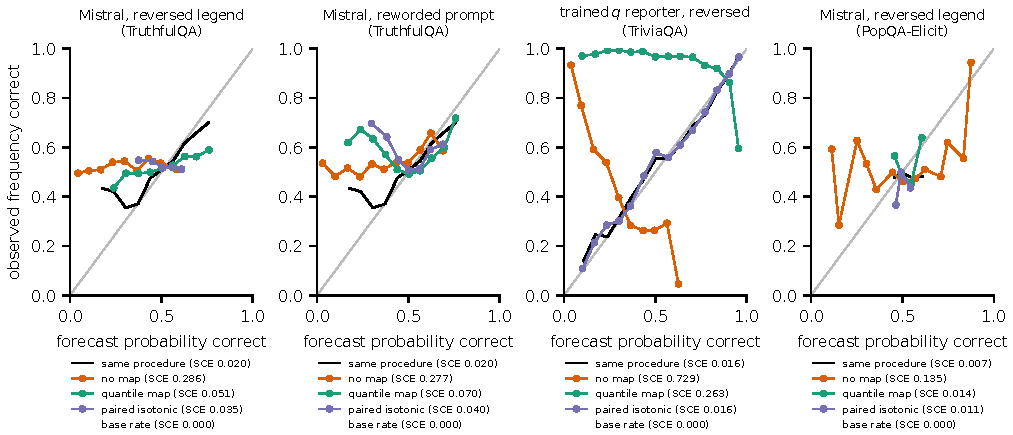
\includegraphics[width=\textwidth]{figs/fig_reliability.pdf}
\caption{Reliability of a forecast fitted under procedure A and applied to procedure-B reports, with
no map, the quantile map and paired isotonic regression, against the same forecast under A (black).
Fifteen equal-width bins, bins with fewer than 20 predictions omitted; SCE from calibration-toolbox,
with a constant forecast at the test base rate as reference (SCE $0$ by construction). Test predictions
pooled over 50 splits (TruthfulQA, \expname{PopQA-Elicit}) or the fixed split (TriviaQA). On PopQA
Mistral's forward report is uninformative, so every forecast stays near $0.5$.}
\label{fig:reliability}
\end{figure*}

\subsection{Pre-set \expname{Granularity} analysis}
The analysis below used a fixed penalty ($C=1$), no report up-weighting and naive intervals; it was
superseded after review by the tuned, controlled and corrected analysis of Section~\ref{sec:e5}, whose
conclusions differ: the direct predictor is not the riskiest choice at small budgets, and the
groups-versus-recalibration contrasts do not survive correction.
\paragraph{Pre-set \expname{Granularity} analysis (superseded).}

(Criteria fixed in a dated protocol note before the run; supplementary material.)
\emph{Data.} Controlled reporting interventions: the three frozen models on 817 TruthfulQA
questions, one label-blind candidate each, under three procedures (forward legend, reversed
legend, reworded prompt). Held-out factual QA: PopQA (7{,}377 questions) with a linear probe as
the confidence report. \emph{Groups}: farthest-first cells on 16 PCA dimensions of the candidate's
frozen hidden state, computed before any confidence prompt. \emph{Forecasters}, all fitted on the
same $n_{\mathrm{lab}}$ labels: R, Platt recalibration of the report per procedure (= one group);
G$_M$, the same with $M$ group intercepts per procedure; GS$_M$, group intercepts shared across
procedures; MC, R multicalibrated over 8 groups $\times$ 4 report quartiles; D, logistic
regression on the 16 representation features and the report. 200 random splits (TruthfulQA), 100
(PopQA); paired differences against R.

\begin{table*}[t]
\caption{Pre-set E5 analysis (superseded): Brier difference against R with naive intervals, fixed penalty. Bold: worse than R.}
\centering\small
\begin{adjustbox}{max width=\textwidth}
\begin{tabular}{lcccc}
\toprule
Brier difference vs.\ R (95\% CI) & $n_{\mathrm{lab}}=60$ & 120 & 180 & 272\\
\midrule
Llama, G$_4$   & $-.003$ & $-.007$ & $-.008$ & $-.009$\\
Mistral, G$_4$ & $\mathbf{+.004}$ & $-.002$ & $-.004$ & $-.005$\\
Qwen, G$_4$    & $-.004$ & $-.008$ & $-.009$ & $-.010$\\
G$_8$ (three models) & $+.005$ to $+.013$ & & & $-.007$ to $-.011$\\
D (three models) & $+.005$ to $+.010$ & $-.014$ to $-.019$ & & $-.030$ to $-.034$\\
MC (three models) & $+.000$ to $+.002$ & & & $-.004$ to $+.003$\\
\midrule
Brier-minimising $M$ (Llama / Mistral / Qwen) & 4 / 1 / 4 & 4 / 4 / 4 & 4 / 8 / 4 & 16 / 8 / 8\\
\bottomrule
\end{tabular}
\end{adjustbox}
\end{table*}
These intervals are naive (they ignore the overlap between splits) and the forecasters used a fixed
penalty; the corrected analysis of Section~\ref{sec:e5} supersedes every interpretive statement made
from this table.

\subsection{Lossless coarsening}
\begin{proposition}[Lossless coarsening]
\label{prop:C}
Let cells $j,k$ have continuous, strictly increasing within-cell score CDFs $F_j,F_k$ with
population $t$-quantiles $q_j,q_k$ and masses $p_j,p_k>0$. Merging them leaves both
children at exact coverage $t$ iff $q_j=q_k$.
\end{proposition}
\begin{proof}
The merged quantile $q_m$ solves $p_jF_j(q_m)+p_kF_k(q_m)=(p_j+p_k)t$. If $q_j=q_k$ this
is solved by $q_m=q_j$ and both children have coverage $t$. If $q_j<q_k$, then
$F_j(q_m)>t>F_k(q_m)$ for the unique solution, which lies strictly between, so one child
over-covers and the other under-covers.
\end{proof}
\subsection{Top-$k$ retrieval and balanced cells}
\label{sec:topk}
With $k>1$ the calibration pool is the union of the calibration rows whose $k$ nearest cells
meet the query's $k$ nearest (each row pooled once). Pools overlap and are query-dependent, so
the Mondrian proof of Theorem~\ref{thm:A} does not transfer; $k=1$ recovers it. Cell MSCE
remains computable; the exact Beta formula of Corollary~\ref{cor:B0} does not.

On the \expname{Trained-Reporters} data (answer-aware reporter, $M=16$, $n_{\mathrm{cal}}=8000$, 50 random re-splits;
descriptive, criteria in a dated addendum): $k=1$ covers $0.900$ (worst pool $0.896$). For
$k=2$ and $k=4$ the average rises to $0.947$ and $0.935$, while the worst query neighbourhood
falls to $0.848$ and $0.766$ (each with about 1{,}150 test rows). Overlapping pools over-cover
on average and under-cover locally; averages hide exactly the failure the partition guarantee
excludes.

\paragraph{Balanced cells.} Power-diagram cells with $\Dfit$-fitted weights reach
exactly equal fit masses but do not help. Against Voronoi cells at matched $M$ on the \expname{Trained-Reporters}
data, the binned forecast's Brier score is worse at $M=8$ (paired difference $+0.0012$
[$0.0011,0.0013$]) and unchanged at $M=16,32$; worst-cell coverage differences have CIs
containing~0. We do not claim a benefit from balancing.

% ---------------------------------------------------------------------
\end{document}
